%%% File encoding: UTF-8
%%% äöüÄÖÜß  <-- keine deutschen Umlaute hier? UTF-faehigen Editor verwenden!
% TODO: CMS durch CRUD-Anwendung erstezen?

%%% Magic Comments zum Setzen der korrekten Parameter in kompatiblen IDEs
% !TeX encoding = utf8
% !TeX program = pdflatex 
% !TeX spellcheck = de_DE
% !BIB program = biber

\documentclass[bachelor,german]{hgbthesis}
% Zulässige Optionen in [..]: 
%   Typ der Arbeit: diploma, master (default), bachelor, internship 
%   Hauptsprache: german (default), english
%%%----------------------------------------------------------

\RequirePackage[utf8]{inputenc}		% bei der Verw. von lualatex oder xelatex entfernen!

\graphicspath{{images/}}    % Verzeichnis mit Bildern und Grafiken
\logofile{logo}				% Logo-Datei = images/logo.pdf (\logofile{}, wenn kein Logo gewünscht)

\bibliography{references}  	% Biblatex-Literaturdatei (references.bib)

%%%----------------------------------------------------------
% Angaben für die Titelei (Titelseite, Erklärung etc.)
%%%----------------------------------------------------------

%%% Einträge für ALLE Arbeiten: -----------------------------
\title{Webkomponenten zur Entwicklung von Serveranwendungen }
\author{Andreas Hahn}
\programname{Medientechnik und -design}
\placeofstudy{Hagenberg}
\dateofsubmission{2018}{02}{28}	% {YYYY}{MM}{DD}

%%% Zusätzlich für eine Bachelorarbeit: ---------------------
\thesisnumber{S1510238020-A}   % Stud-ID, z.B. 1310238045-A  
% (A = 1. Bachelorarbeit)
\semester{Sommersemester 2017} 
\coursetitle{Bachelorarbeit 1} 
\advisor{Rimbert Rudisch-Sommer}

%%% Restriktive Lizenformel anstatt CC (nur für Typ master) -
%\strictlicense

%%%----------------------------------------------------------
\begin{document}
%%%----------------------------------------------------------

%%%----------------------------------------------------------
\frontmatter                    % Titelei (röm. Seitenzahlen)
%%%----------------------------------------------------------

\maketitle
\tableofcontents

\chapter{Vorwort} 	% engl. Preface


Dies ist \textbf{Version \hgbthesisDate} der \latex-Dokumentenvorlage für 
verschiedene Abschlussarbeiten an der Fakultät für Informatik, Kommunikation
und Medien der FH Oberösterreich in Hagenberg, die mittlerweile auch 
an anderen Hochschulen im In- und Ausland gerne verwendet wird.

Während dieses Dokument anfangs ausschließlich für die Erstellung
von Diplomarbeiten gedacht war, sind nunmehr auch  
\emph{Masterarbeiten}, \emph{Bachelor\-arbeiten} und \emph{Praktikumsberichte} 
abgedeckt, wobei die Unterschiede bewusst gering gehalten wurden.

Die Verwendung dieser Vorlage ist jedermann freigestellt und an
keinerlei Erwähnung gebunden. Allerdings -- wer sie als Grundlage
seiner eigenen Arbeit verwenden möchte, sollte nicht einfach
("`ung'schaut"') darauf los werken, sondern zumindest die
wichtigsten Teile des Dokuments \emph{lesen} und nach Möglichkeit
auch beherzigen. Die Erfahrung zeigt, dass dies die Qualität der
Ergebnisse deutlich zu steigern vermag.

Der Quelltext zu diesem Dokument sowie das zugehörige
\latex-Paket sind in der jeweils aktuellen Version online
verfügbar unter
%
\begin{itemize}
\item[]\url{https://github.com/Digital-Media/HagenbergThesis}.
\end{itemize}
%
Trotz großer Mühe enthält dieses Dokument zweifellos Fehler und Unzulänglichkeiten
-- Kommentare, Verbesserungsvorschläge und passende Ergänzungen
sind daher stets willkommen, am einfachsten per E-Mail direkt an mich:
\begin{itemize}
\item[]%

Dr.\ Wilhelm Burger, Department für Digitale Medien,\newline
Fachhochschule Oberösterreich, Campus Hagenberg (Österreich)\newline
\nolinkurl{wilhelm.burger@fh-hagenberg.at}
\end{itemize}

\noindent
Übrigens, hier im Vorwort (das bei Diplom- und Masterarbeiten üblich, bei Bachelorarbeiten 
aber entbehrlich ist) kann kurz auf die Entstehung des Dokuments eingegangen werden.
Hier ist auch der Platz für allfällige Danksagungen (\zB an den Betreuer, 
den Begutachter, die Familie, den Hund, \ldots), Widmungen und philosophische 
Anmerkungen. Das sollte allerdings auch nicht übertrieben werden und sich auf 
einen Umfang von maximal zwei Seiten beschränken.




 % Optional. Ggf. weglassen
\chapter{Kurzfassung}

Webkomponenten tragen zur Atomisierung der Webprogrammierung bei, da diese den WebentwicklerInnen die Möglichkeiten bieten, bestehende HTML Elemente zu erweitern und eigene zu kreieren. Dieser unscheinbarer Zusatz ermöglicht ProgrammiererInnen ihre Software aus mächtigen, zusammengesetzten Komponenten zu erstellen.
Diese Bachelorarbeit konzipiert ein Gerüst aus Webkomponenten in Kombination mit anderen gängigen Webtechnologien, welche die Erstellung einer Serveranwendung weitgehend mit Webkomponenten ermöglicht und testet dieses anhand eines für diese Arbeit entwickelten Prototypen.

		
\chapter{Abstract}

\begin{english}
	Webcomponents aim towards atomarizing web programming by giving developers the possibility to extend already exisitng HTML elemnts and to create own components. This modest addition enables programmers to build their software out of combined, powerfull components.
	This bachelor thesis focuses on the development of a framework of web components in combination with other popular web technologies to develop a server application using webcomponents. This framework will then be evaluated based on a prototype implemented as a project in the fifth semester.
	
	
\end{english}
			

%%%----------------------------------------------------------
\mainmatter          % Hauptteil (ab hier arab. Seitenzahlen)
%%%----------------------------------------------------------

\chapter{Einleitung}

\section{Motivation}

Die Idee, die Webprogrammierung komponentenorientiert zu gestalten, gibt es seit 1998 \cite{microsoft-webcomponents}. Jedoch hat sich diese Idee, bis heute, nicht zu einem Web-Standard weiterentwickelt.
Seit einigen Jahren gibt es dazu wieder Ansätze, welche von größeren Firmen, wie beispielsweise Google mit Angular\footnote{https://angular.io/} oder Facebook mit React\footnote{https://facebook.github.io/react/}, mittels eigens entwickelten komponentenbasierten Frameworks versuchen, die komponentenorientierte Webentwicklung voran zu treiben. 
Allerdings ist seit neuestem die grundlegende Idee der nativen Webkomponenten\footnote{https://www.webcomponents.org/}, welche künftig nur als Webkomponenten bezeichnet werden, zurück. Da diese, sobald gängige Webbrowser alle Technologien von Webkomponenten -- HTML Imports, Templates, Custom Elements, Shadow DOM -- unterstützen, einen weiteren Schritt in standardisierte, wiederverwendbare und unabhängige Webbausteine bedeutet. Zur Zeit ist es noch nicht, oder erschwert möglich, clientseitig und  serverseitig auf Webkomponenten zu setzen.
Diese Bachelorarbeit beleuchtet jene Problematik und stellt Lösungsvorschläge anhand einer konkreten CRUD-Anwendung dar.


\section{Forschungsfrage}
\label{sec:hintergrund}

Eine CRUD-Anwendung (Create, Read, Update, Delete) ist eine Anwendung, welche die vier grundlegenden Operationen implementiert, um Daten zu manipulieren. BenutzerInnen können durch eine Benutzeroberfläche Datensätze erstellen, lesen, bearbeiten und löschen. 
Angular oder React wären für die Umsetzung einer solchen Anwendung geeignet. Aus heutiger Sicht zählen diese Technologien zu den gängigsten Frameworks und werden von zahlreichen EntwicklerInnen stetig verbessert.
Diese besagten Frameworks sind mit einer steilen Lernkurve behaftet und benötigen Zeit um sich damit vertraut zu machen.

Im Gegensatz dazu sind Webkomponenten logisch deklariert und bauen lediglich auf Kenntnissen von nativem HTML, CSS und Javascript auf. Die Unterstützung wird noch nicht von jedem Browser gewährleistet und verursacht aus diesem Grund ein Zögern bei einigen EntwicklerInnen, um komplett auf Webkomponenten zu setzen.
Google hat mit Polymer\footnote{https://www.polymer-project.org/} eine Javascript-Bibliothek geschaffen, welche die Kreierung und Nutzung von Webkomponenten ungemein vereinfacht. Darüber hinaus nutzt diese Bibliothek Polyfills, die Funktionen, welche Polymer benötigt, bei Bedarf liefert und wird dadurch nicht nur in allen gängigen Webbrowsern -- Chrome, Firefox, Edge, Safari --  sondern auch in deren älteren Versionen, die die notwendigen Funktionen nicht implementiert haben, unterstützt \cite{polymer-compatibility}. Native Unterstützung ist bereits bei den meisten Browserherstellern in Entwicklung und würde Polyfills überflüssig machen.\newline
\newline Aus diesen Ansätzen ergibt sich folgende Forschungsfrage für diese Bachelorarbeit:

\begin{quote}
Wie muss eine Webanwendung programmatisch konzipiert werden, um die grundlegenden Funktionen weitgehend mittels server- und clientseitigen Webkomponenten zu realisieren?
\end{quote}

\section{Methodik}

Um diese Frage zu beantworten, soll die Bachelorarbeit als eine Kombination von Literaturarbeit und praktischer \bzw prototypischer Umsetzung realisiert werden.

Zunächst soll aus bestehender Literatur (erweiternd zu Abschnitt \ref{sec:hintergrund}) erörtert werden, wie mit dem Thema der Webkomponenten und mit komponentenorientierten Frameworks umgegangen wird. Gemeinsame Faktoren sollen daraus extrahiert werden und als Grundlage für ein eigenes, theoretisches Konzept dienen. Die Vorteile und Limitierungen von Webkomponenten werden dabei erörtert. Dieses Konzept soll schlussendlich eine Liste von Kerntechniken enthalten, welche die Umsetzung einer CRUD-Anwendung mittels Webkomponenten ermöglicht.

Überprüft werden soll die Anwendbarkeit dieses Konzepts, durch einen eigenen, im Rahmen dieser Arbeit entwickelten Prototypen.

\section{Erwartete Ergebnisse}

Als konkretes Ergebnis wird ein Gerüst mit Webkomponenten erstellt, welches als Grundlage für die Erstellung einer Webanwendung dienen soll. Es wird erwartet, dass sich solche konkreten Techniken finden und umsetzen lassen.

Bei der praktischen Umsetzung der Webkomponenten in einer CRUD-Anwendung wird ebenfalls eine positive Evaluierung erwartet, da es bereits erfolgreiche Konzepte basierend auf server- und clientseitigen Webkomponenten gibt und somit auf deren Erfahrungen aufgebaut werden kann.

\section{Aufbau der Arbeit}
Im ersten Teil dieser Arbeit werden technische Grundlagen bezüglich Webkomponenten erörtert, und wie eine REST-Architektur aufgebaut ist. Im Kapitel danach werden State of the Art Technologien besprochen. Im Anschluss wird das grundlegende Konzept der praktischen Arbeit erläutert. Im fünften Kapitel wird die konkrete Implementierung der Webanwendung behandelt. Im darauffolgenden Abschnitt -- Evaluierung -- werden objektiv die Vor- und Nachteile, der im Fokus stehenden Technologie, aufgezeigt. Im siebten und letzten Kapitel wird  zusammenfassend die persönliche Meinung, bezüglich der Thematik, einfließen. 
\chapter{Technische Grundlagen}

\section{Webkomponenten}
\label{cha:webcomponents}
Wie der Name -- Webkomponente -- suggeriert, ermöglicht diese Technologie die Webentwicklung in kleinere, wiederverwendbare, modulare Container zu "`komponentisieren"'.  Der klare Vorteil besteht darin, dass diese Komponenten, unabhängig von einem Framework, vollständig mit "`vanilla"' HTML, CSS und Javascript kreiert werden können, und wie in Kap.~\ref{cha:component_usage} erwähnt, Code wartbar machen.
\newline
Webkomponenten bestehen aus 4 separaten W3C Standards\footnote{\url{https://www.w3.org/standards/techs/components\#w3c\_all}}:
\begin{itemize}
	\item Custom Elements - APIs um neue HTML Elemente zu definieren
	\item HTML Imports - deklarative Methode um HTML Dokumente in andere zu importieren
	\item HTML Templates - <template>-Element, welches Dokumenten eigenen DOM ermöglicht
	\item Shadow DOM - DOM und Styling abkapseln
\end{itemize}
An einer Standardisierung der Webkomponenten wird bereits Seiten der W3C gearbeitet. Mehr dazu findet sich in \cite{w3c-components}. Jedoch um diese derzeitig in allen größeren Browsern zu nutzen, gibt es sogenannte Polyfills \cite{polyfill}. Dieses Polyfill ist ein Codestück, welches Technologie zur Verfügung stellt, die der Browser nicht nativ unterstützt.

\subsection{Custom-Elements}
Custom-Elements gibt den EntwicklerInnen die Fähigkeit, eigene, voll funktionsfähige DOM-Elemente zu erstellen, existierende HTML-Tags zu erweitern und/oder von anderen EntwicklerInnen erstellte Elemente zu nutzen.  

Diese Spezifikation ist Teil eines größeren Projekts, das Internet zu rationalisieren, im Hinblick auf EntwicklerInnen zugänglichen Schnittstellen, wie beispielsweise die Custom-Elements-Definition. Jedoch gibt es immer noch Limitierungen, welche das komplette Potenzial -- semantisch und funktional -- einschränken, um das Verhalten bestehender HTML-Elemente vollständig, mit selbst erstellten Elementen, zu beschreiben. Mehr dazu findet sich in \cite{custom-elements}.

\begin{program}[!htbp]
\caption{Exemplarische Definition eines Custom-Elements}
\begin{JsCode}
class HelloWorld extends HTMLElement {...};
customElements.define("hello-world", HelloWorld);
\end{JsCode}
\end{program}
\subsection{HTML Import}
HTML Importe ermöglichen das Inkludieren und Wiederverwenden von HTML-Dokumenten in anderen Dokumenten. Dieser Import beinhaltet all jene Elemente, die in einem HTML-Dokument definiert sind (Javascript, CSS, HTML, ...). 
Diese Möglichkeit, mehrere Technologien in einem Import, sozusagen eine URL, zu bündeln, ist klein, aber wesentlich. Aktuell wird es von kaum einem Browser, außer Chrome 62,  unterstützt\footnote{\url{https://caniuse.com/\#search=HTML\%20Import}}. Mehr über \emph{HTML Imports} in \cite{html-imports}.

\begin{program}[!htbp]
\caption{Exemplarischer HTML Import}
\begin{JsCode}
<link rel="import" href="hello-world.html">
\end{JsCode}
\end{program}
\subsection{HTML Templates}
Das Template Element kapselt Bestandteile einer Webseite ab, welche durch Skripte geklont und zur Laufzeit in das Dokument eingefügt werden können. Die Darstellung des Elements ist beim Laden und erstmaligen rendern der Seite leer, und wird zur Laufzeit mit Javascript gerendert. Dieses Element kann als Inhaltsplatzhalter angesehen werden, welcher für spätere Verwendung gespeichert wird. 

\begin{program}[!htbp]
\caption{Exemplarisches HTML Template}
\label{prog:html-template}
\begin{JsCode}
<template id="template">
	<p>Hello World!</p>
</template>
\end{JsCode}
\end{program}
Das p-Element, wie im Programm~\ref{prog:html-template} gezeigt, ist kein Kindelement des Template Elements im DOM. Es ist ein Kind des DocumentFragment, welches vom content IDL Attribut des Templates zurückgegeben wird, wie in \cite{html-templates} erläutert.

\subsection{Shadow DOM}
Der Shadow Dom bietet eine API zur Erstellung eines separaten Baumes, Shadow Tree genannt, welcher an ein Element angehängt werden kann.
Das bringt die Abkapselung von DOM-Elementen und CSS mit sich. Beispielsweise kann unorganisierter CSS-Code von einem Bereich in den anderen durchsickern und wiederum einen Konflikt erzeugen, welcher unbeabsichtigtes Verhalten hervorbringt. 

Shadow DOM löst dieses Problem durch Isolierung der CSS-Bereiche und Abkapselung des DOM. 
Gemeinsam mit der Custom-Element-API ermöglicht es das Schreiben von Komponenten mit in sich geschlossenem HTML, CSS und Javascript.

Um den Shadow DOM eines Elements zu erstellen muss diesem lediglich der Shadow Root angehängt werden.
\begin{program}[!htbp]
\caption{Exemplarisches HTML Template}
\label{prog:shadow-dom}
\begin{JsCode}
const p = document.createElement('p');
const shadowRoot = p.attachShadow({mode: 'open'});
\end{JsCode}
\end{program}

\section{Representational State Transfer  API}
In diesem Abschnitt wird der Begriff der \begin{english}
Representational State Transfer (REST)
\end{english} Architektur, welcher von Roy Thomas Fielding im Jahre 2000 eingeführt wurde, beschrieben \cite{rest}.
Der als REST bezeichnete Architekturansatz beschreibt die grundlegenden Regeln, wie verteilte Systeme miteinander kommunizieren können.
Fielding hat für diese Architektur Restriktionen zusammengefasst, welche in dem folgendem Abschnitt erläutert werden.
\subsection{Restriktionen}
\subsubsection{Null Stil}
Der Null Stil beschreibt den Status eines Systems, wenn jenes keine Abgrenzungen der enthaltenen Komponenten aufweist. Von diesem Status weg wird REST definiert. 
\subsubsection{Client-Server}
Nach dem Client-Server-Architektur Stil werden Aufgabenbereiche auf Client und Server aufgeteilt. Meist wird vom Client eine Aufgabe gestellt, und diese vom Server verarbeitet. 
\subsubsection{Zustandslosigkeit}
Jegliche REST-Zugriffe sind zustandslos. Das bedeutet, jede Anfrage enthält alle benötigten Informationen, die der Endpunkt braucht, um diese zu verstehen und zu verarbeiten. Unabhängig davon, wer oder was die Anfrage getätigt hat.  
\subsubsection{Einheitliche Schnittstelle}
Eine standardisierte Schnittstelle soll durch die Trennung der Zuständigkeiten die Einfachheit fördern, sowie die darunter liegende Implementierung und Kommunikation verbergen. 
\subsubsection{Caching}
Die effizienteste Netzwerkanfrage ist jene, die das Netzwerk nicht benutzt.
Soll heißen, dass eine wiederverwendbare, gecachte Antwort die Performanteste ist. 
\subsubsection{Stufen Systeme}
Das Zielsystem soll, wie in Kap.~\ref{cha:webapplication_structure} weiter behandelt, mit n-Stufen aufgebaut sein, damit der Anwender lediglich auf eine Schnittstelle, einer Stufe, zugreifen muss, und die anderen verborgen bleiben können.

\subsection{Praxis}
In der Praxis wird das REST-Paradigma bevorzugt per HTTP/S realisiert. Services werden über eine URL/einen URI angesprochen. Wie eine Anfrage bearbeitet werden soll, kann per HTTP-Methode (GET, POST, PUT, \etc) verfeinert werden. 
%TODO Wie wird bisher serveranwendungen erstellt? 
% CMS Systeme: WordPress, TYPO3
%oder symfony, laravel
\chapter{State of the Art}
\label{cha:StateOfTheArt}
MEAN Stack ?
\chapter{Grundlegendes Konzept}

\section{Aufbau einer Webanwendung}
\label{cha:webapplication_structure}

Das Konzept der Schichtenarchitektur ist in der Softwareentwicklung eine Client-Server-Architektur, welche die Darstellung, Anwendungslogik und Datenverwaltung physikalisch trennt.  
Das Konzept der abgestuften Architektur bei der Anwendungsentwicklung lässt sich von einem 1-Stufen-Ansatz bis hin zu einem n-Stufen-Ansatz einteilen. Jeder dieser Ansätze hat seine Vorzüge, doch für eine webbasierte Anwendung eignet sich der n-Stufen-Ansatz. Das Grundkonzept einer solchen Architektur besteht darin, eine Anwendung in unabhängige Ebenen mit definierten Rollen aufzuteilen.
Die mehrstufige Anwendungsarchitektur ermöglicht es den EntwicklerInnen flexible, wiederverwendbare und austauschbare  Anwendungskomponenten zu erstellen, welche zu einer Schichtenanwendung verknüpft werden können, ohne die komplette Endanwendung umschreiben zu müssen.
Diese mögen sich auf der selben Maschine befinden, werden aber meist auf unterschiedliche ausgelagert \cite{wiki-ntier-architecture}.

Beispielsweise sind bei dem 1-Stufen-Ansatz alle für die Anwendung relevanten Funktionen -- Darstellung, Logik, Datenverwaltung, \etc -- auf der Client-Maschine vereint. Durch die Limitierung, dass die komplette Software auf einem Gerät betrieben wird und die daraus folgenden Skalierungsprobleme, ist dieser Ansatz kaum für Webanwendungen geeignet.
Der gebräuchlichste Stufenansatz ist der 3-stufige, siehe Abb.~\ref{fig:3-stufen-architektur}, welcher in der Regel Darstellung, Anwendungslogik und Datenverwaltung entkoppelt. Ein Webbrowser, zur Anzeige der Benutzeroberfläche, wäre zum Beispiel die erste Stufe. Ein Webserver, welcher die Logik ausführt, die Zweite und als dritte Ebene, zur Datenverwaltung, käme eine Datenbank in Frage. 

Obwohl der 3-Stufen-Ansatz die Skalierbarkeit erhöht und eine Trennung der Anwendungslogik von den Anzeige- und Datenverwaltungsschichten einführt, trennt er die Anwendung nicht wirklich in spezialisierte Schichten. Für Prototyp- oder einfache Webanwendungen kann eine dreistufige Architektur ausreichen. Bei komplexen Anforderungen an solche Anwendungen ist ein 3-stufiger Ansatz jedoch in mehreren Schlüsselbereichen, einschließlich Flexibilität und Skalierbarkeit, unzureichend, und es wäre sinnvoll, einen n-Stufen-Ansatz zu wählen \cite{nTier-architecture}.

Der größte Nachteil von diesen Ansätzen ist der zusätzliche Overhead-Aufwand  und eine höhere Latenz, was wiederum die der NutzerInnen wahrgenommen Geschwindigkeit mindert.

Die Trennung von Logik ist in der Webentwicklung ein wesentliches Konzept. Wie in diesem Kapitel die Abstraktion durch Stufen, oder Ebenen, wird im folgenden Kapitel \ref{cha:component_usage} die Trennung von Logik, mittels Komponenten, behandelt.

\begin{figure}
	\centering
	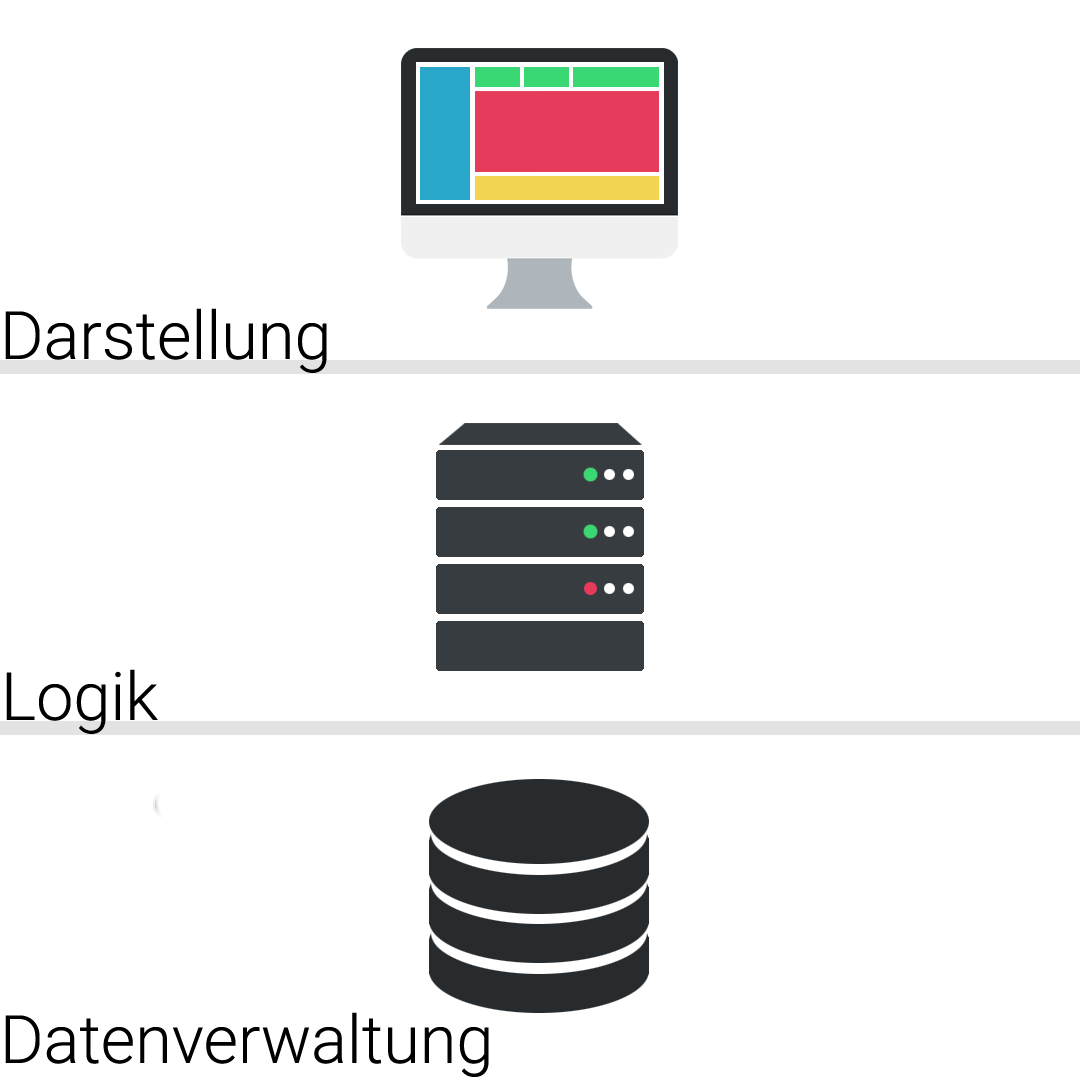
\includegraphics[width=0.5\linewidth]{images/3-stufen-architektur}
	\caption{3-Stufen-Architektur}
	\label{fig:3-stufen-architektur}
\end{figure}

\section{Verwendung von Komponenten im Web}
\label{cha:component_usage}
%TODO How to gender EntwicklerIn, der/des entwicklers?
%TODO Darf man das Beispiel 1:1 reproduzieren ?
Das Web besteht aus Bausteinen, sogenannten Elementen. Wenn EntwicklerInnen beispielsweise einen Link mittels einem a-Tag nutzen, wird erwartet, dass dieser sich wie ein Link-Element verhält. Dieses Element hat seine eigene standardmäßige blaue Farbe, einen Handzeiger bei hover und vor allem die Funktionalität, dass bei einem Klick auf das Element zu einer neuen URL weitergeleitet wird. Dieses Verhalten und Styling wird ohne jegliches einwirken des/der EntwicklerIn bereitgestellt. Jedes HTML Element funktioniert nach diesem Prinzip, welches HTML Code einfacher zu schreiben, aber auch verständlicher macht.
Durch Kombination solcher Elemente, mit eigens definierten Stylesheets können komplexere Gerüste aus HTML Elementen, mit komplexeren CSS/Javascript entstehen.

Damit nicht ein/eine EntwicklerIn die komplette Struktur im Kopf behalten muss, und bei Problemen nur diese/r das aufgetretene Problem beheben kann, hat sich bewehrt, Code in kleine, überschaubare Teile herunter zu brechen, in Einheiten, welche das gesamte Gerüst wartbar machen. Diese Teile können einfachere Funktionen, Module, Komponenten oder aber viele andere Ansätze sein, welche komplexe Strukturen in atomare Einzelteile aufteilen \cite{components-benefit}.

Um also die Definition der, in dieser Arbeit fokussierten Technologie -- einer Komponente -- zusammen zu fassen: Eine entkoppelte Sammlung von Funktionalität oder Prozessen und Logik, mit einer verständlichen Schnittstelle oder API um des Komponenten Funktionalität abzurufen.

\section{Anforderung an die komponentenorientierte Webanwendung}

\section{Eigene Idee, technisches Design}

\chapter{Implementierung der Webanwendung}

Die AnwenderInnen sollen zu Beginn Datensätze anlegen können. Im Prototypen wurde das Datenmodell von Personen mit Benutzername, E-Mail und Passwort herangezogen.
Nachdem die AnwenderInnen das Formular für eine Person ausgefüllt haben, kann dieser Datensatz angelegt werden. Nach elementaren Validierungen werden die Daten an den Server übermittelt. Dieser speichert diese wiederum in der Datenbank ab. 
In der Listenansicht sehen die AnwenderInnen alle bereits angelegten Personen in einer Tabelle und per Klick auf den Namen wird zur Detailansicht weitergeleitet. Hier wird ein Formular mit den Nutzerdaten ausgefüllt, welche verändert und aktualisiert werden können.   
Auf der Detailseite findet sich ebenso ein Lösch-Knopf, um eine bestehende Person zu entfernen. Dadurch sind alle CRUD-Operation abgedeckt.
\section{Umsetzung mit Dependencies Electron / Scram-Engine}
Um die Nutzung von Webkomponenten am Server zu ermöglichen, werden zwei konkrete Technologien benötigt, da Webkomponenten grundsätzlich nur im Browser funktionieren.
\subsection{Electron}
Electron ist ein Framework, um native Cross-Plattform-Applikationen mit Web-Technologien wie JavaScript, HTML und CSS zu erstellen. Es basiert auf dem Chromium\footnote{https://www.chromium.org/} Webbrowser und Node.js.
\subsection{Scram-Engine}
\label{cha:scram-engine}
Das Scram-Engine-Projekt, erarbeitet von Jordan Last, ermöglicht es, eine HTML-Datei einem vorkonfigurierten Electronstartscript mit minimalem Aufwand, zur Verfügung zu stellen. Es wird lediglich Electron von der Kommandozeile aufgerufen und eine Startdatei mitgegeben. Die Vorkonfiguration vereinfacht das Arbeiten mit Electron durch beispielsweise das Anbieten von Kommandozeilenargumenten, um das Electronfenster zu verstecken, und somit das bequeme Starten von serverseitigen Anwendungen aus der Kommandozeile heraus.
Electron ist notwendig, da es Chromium mit Node.js kombiniert. Die Scram-Engine nutzt Chromiums Fähigkeit, Webkomponenten in einen interaktiven DOM zu parsen, welcher manipuliert werden kann. Diese Webkomponenten können dadurch jeglichen Node.js Code nutzen und haben die Möglichkeit mit dem Betriebssystem zu interagieren, Datenbankaufrufe zu tätigen, prinzipiell alles, was Node.js möglich ist.
Ein reiner Node.js Server würde nicht ausreichen, da dieser HTML, Custom-Elemente oder Webkomponenten generell nicht parsen kann.
Durch die Kombination der beiden Technologien können Webkomponenten weitaus mehr leisten, als in einem Webbrowser.

Da universelle Webkomponenten auf Electron als deren Plattform angewiesen sind, muss das System, welches diese betreibt, relativ leistungsstark sein. Jordan Last arbeitet an einer Lösung, um die Electron-Abhängigkeit -- und dadurch die Chromium-Abhängigkeit -- loszuwerden. Jegliche Interessenten, die an dieser Optimierung mitwirken möchten, können ihn kontaktieren\footnote{https://github.com/lastmjs}.

\section{Implementierung der Komponenten}
Der für diese Arbeit entwickelte Prototyp kann in die Hauptteile Frontend und Backend eingeteilt werden. Wobei das Backend nochmals in Server und Datenbank unterteilt wird. 

\subsection{Frontend}
Im Frontend wurde hauptsächlich auf bereits vorhandene Webkomponenten aufgebaut. Es wurden Standard HTML-Elemente durch paper-input Elemente\footnote{https://www.webcomponents.org/collection/PolymerElements/paper-input-elements} ersetzt, um ein abgestimmtes Gesamtbild zu erzeugen, ohne sich auf das Design konzentrieren zu müssen. So wurde bei dem Anlegen einer neuen Person, wie in Abb. \ref{fig:user_create} ersichtlich, auf <paper-input> Elemente mit einem <iron-icon> Element gesetzt. Das Aktualisieren eines Nutzers ist das selbe Formular, lediglich mit anderen <paper-button> Komponenten. Die Auflistung, aller bereits erstellten Personen, wurde durch ein <paper-datatable-api> Element erstellt. Jegliche Kommunikation zwischen Frontend und Backend wurde über eine REST-API gehandhabt. Die Anfragen wurden durch <iron-ajax> Komponenten vollzogen, welche eine Webkomponente für einfache ajax-Anfragen ist.
\begin{figure}
	\centering
	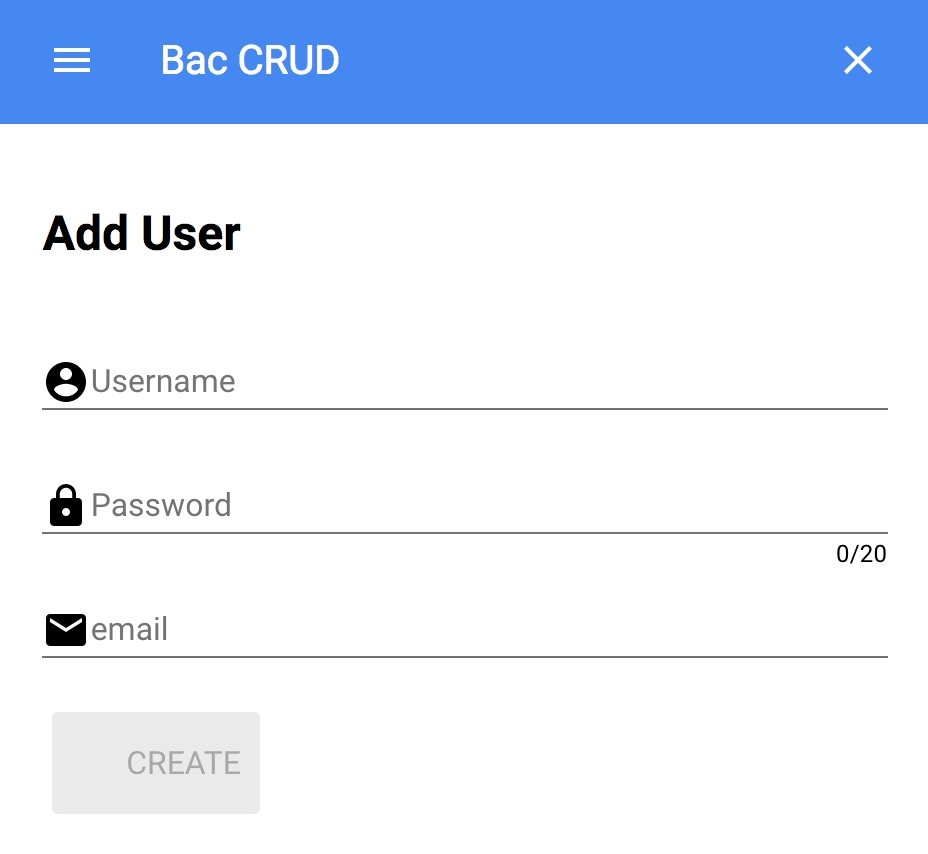
\includegraphics[width=0.5\linewidth]{images/user_create.jpeg}
	\caption{User erstellen}
	\label{fig:user_create}
\end{figure}

\begin{figure}
	\centering
	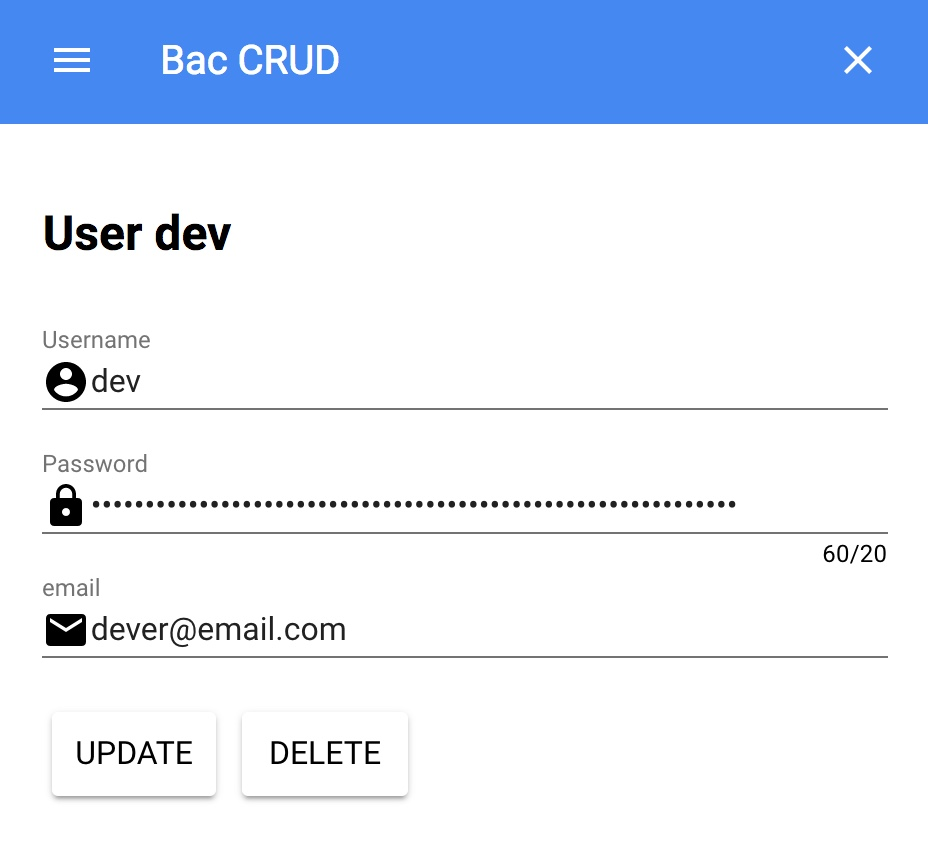
\includegraphics[width=0.5\linewidth]{images/user_update.jpeg}
	\caption{User bearbeiten}
	\label{fig:user_update}
\end{figure}

\begin{figure}
	\centering
	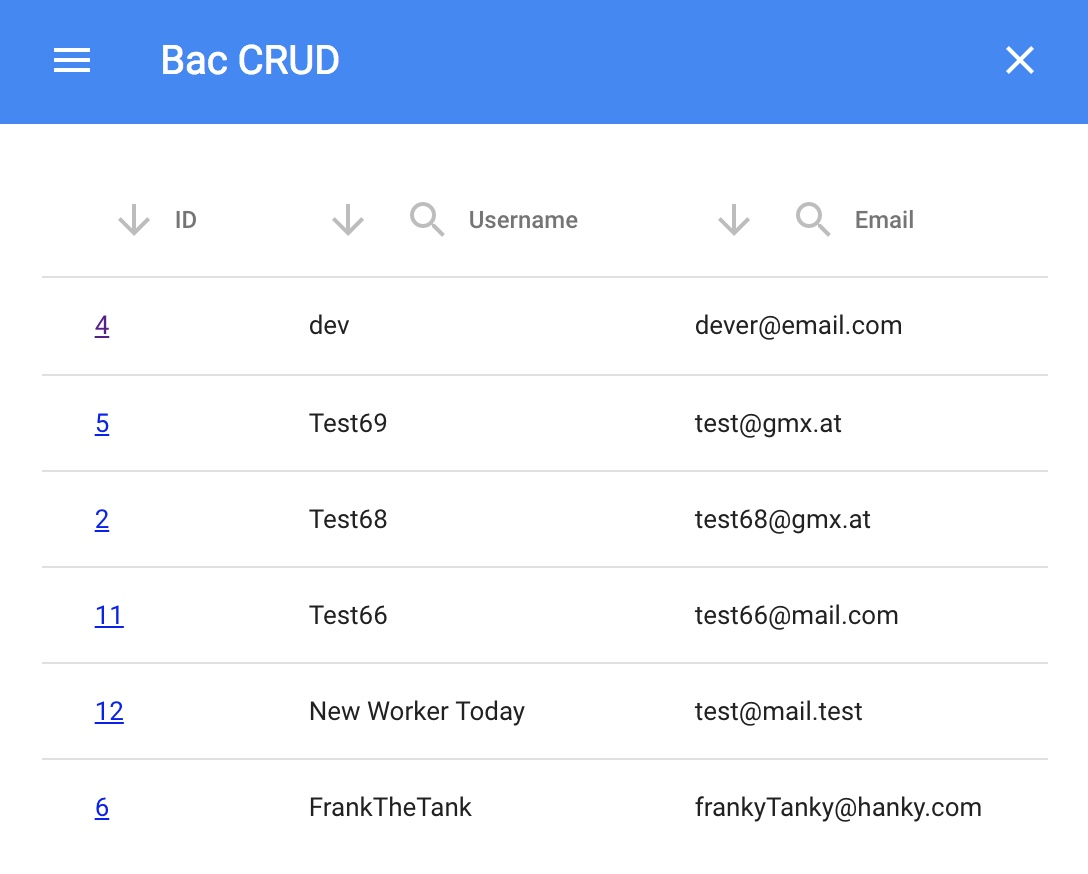
\includegraphics[width=0.5\linewidth]{images/user_list.jpeg}
	\caption{User Liste}
	\label{fig:user_list}
\end{figure}

\subsection{Server}
Ein Node.js Server kann mit Webkomponenten, wie im Programm \ref{prog:server-config} abgekürzt ersichtlich, konfiguriert und funktionstüchtig eingesetzt werden. Durch <express-app>, <express-config>, <express-middlesware> und <express-router> mit <express-route> Komponenten\footnote{https://github.com/scramjs/express-web-components} kann die komplette Serverumgebung aufgesetzt werden.

In dieser Serveranwendung sind alle Endpunkte und Middlewares, welche die Express-Anwendung manipulieren, unter einer <express-app> Webkomponente  verschachtelt. In der Reihenfolge, wie die Middlewares definiert werden, werden diese auch in die Anwendung eingepflegt. In einem <express-router> Element können ebenfalls <express-route> Elemente und Middlewares verschachtelt, und so komplexe Routen-System erstellt werden.

Anstatt dass REST-Routen in Javascript imperativ definiert, können diese deklarativ in HTML zusammengesetzt werden. Es wird so eine visuelle Hierarchie der vorhanden Routen erstellt. Durch die Visualisierung mit HTML behält man nicht nur den Überblick, es ist auch einfacher zu verstehen als das Äquivalent in Javascript. Hier wird beispielsweise im Programm \ref{prog:route-config} der \textit{indexHandler}(siehe Programm \ref{prog:indexHandler}) als \textit{Callback} an ein <express-middleware> Element übergeben, welches eine Methode(\textit{get}) und einen Pfad(\textit{/})  besitzt. Diese Middleware befindet sich unter dem <express-router> mit der Basisroute als Pfad. Das bedeutet, dass dieser Router für seinen Pfad unter sich Routen haben kann, die ebenso einen Pfad besitzen. Da der \textit{indexHandler} auf die Basisroute angewendet werden soll, wird dieser Middleware ebenfalls die Basisroute als Pfad mitgegeben. Nach diesem Prinzip können jegliche verschachtelte Routen erstellt werden. Wobei Subrouten immer unter der übergeordneten Route verschachtelt werden sollen. So soll die Route \textit{/index/list} unter dem Router für die Route \textit{/index} als Route \textit{/list} geschachtelt werden.

Die gezeigte Route im Code  \ref{prog:route-config} ist rein zur Definition, welche URL, welche Seite rendern soll. Für REST-Anfragen, die Daten aus der Datenbank manipulieren, wurde eine eigene Komponente <db-router> erstellt, welche alle relevanten Datenbankanfragen über zuvor definierte Routen verarbeitet. Diese Komponente, welche selber <express-router> Elemente implementiert, kapselt so Datenbank spezifische Endpunkte von der Serverkonfiguration ab. Dieser <db-router> ist, ebenso wie ein <express-router> Element, ein Kind der <express-app> Komponente. Ersichtlich im Programm \ref{prog:server-config}.

\begin{program}
\caption{Exemplarische Express-App mit Webkomponenten}
\label{prog:server-config}
\begin{HtmlCode}
<express-app port="3000">
	<express-config callback="[[staticMW]]"></express-config>
	<express-middleware callback="[[bodyParserMW]]"></express-middleware>
	<express-router path="/">
	<express-middleware method="get" path="/" callback="[[indexHandler]]"></express-middleware>
	</express-router>
	<db-router></db-router>
</express-app>
\end{HtmlCode}
\end{program}

\begin{program}
\caption{Indexroute-Konfiguration mit Webkomponenten}
\label{prog:route-config}
\begin{HtmlCode}
<express-router path="/">
	<express-middleware method="get" path="/" callback="[[indexHandler]]"></express-middleware>
</express-router>
\end{HtmlCode}
\end{program}

\begin{program}
\caption{indexHandler Funktion}
\label{prog:indexHandler}
\begin{HtmlCode}
indexHandler(req, res) {
	res.sendFile(path.resolve('./client/index.html'));
}
\end{HtmlCode}
\end{program}

\subsection{Datenverwaltung}
Der im Programm \ref{prog:server-config} ersichtliche <db-router> verarbeitet jegliche Datenbank spezifischen Anfragen und triggert <db-query> Komponenten, um Daten der Datenbank zu manipulieren. Siehe Programm \ref{prog:db-query}. Diesem <db-query> Element wird durch Kindelemente gesagt, was es für Abfragen tätigen soll. Besitzt das <db-query> Element beispielsweise lediglich ein <db-find> Element, wird davon ausgegangen, dass ein Datensatz von der Datenbank gesucht und zurückgegeben werden soll. Besitzt es aber zusätzlich zu dem <db-find>, ein <db-delete>, so wird das <db-query> Element nicht den gefunden Datensatz zurückgeben, sondern löschen. 
 
\begin{program}
\caption{Datenverwaltung mit Komponenten}
\label{prog:db-query}
\begin{HtmlCode}
<db-query id="queryListUsers" db-model="[[userModel]]">
	<db-find></db-find>
	<db-sort sort2-query="{{_sort}}" sort-query="[[_sort]]" sort-property="username"
		sort-direction="asc"></db-sort>
</db-query>
	
<db-query id="queryUserDetails" db-model="[[userModel]]">
	<db-find find-query="[[findUserQuery]]"></db-find>
</db-query>
	
<db-query id="querySaveUser" db-model="[[userModel]]">
	<db-save save="[[newUser]]"></db-save>
</db-query>
	
<db-query id="queryUpdateUser" db-model="[[userModel]]">
	<db-find find-query="[[findUserQuery]]"></db-find>
	<db-save save="[[updateUser]]"></db-save>
</db-query>
	
<db-query id="queryDeleteUser" db-model="[[userModel]]">
	<db-find find-query="[[findUserQuery]]"></db-find>
	<db-delete></db-delete>
</db-query>
\end{HtmlCode}
\end{program}

\subsubsection{DB Query Komponente}
Um die interne Arbeitsweise zu verdeutlichen, wird die im Zuge dieser Arbeit entwickelte Webkomponente erläutert. Der exakte Programmcode kann auf GitHub nachgelesen werden\footnote{https://github.com/drdreo/webcomponent-cms/blob/master/server/components/db-query.html}. 
Als Parameter benötigt das <db-query> Element eine eindeutige ID, welche zum Auslösen der Abfrage benötigt wird, und das zugehörige  Datenbankmodell -- da dieses Element für mongoDB mit mongoose entworfen wurde.
Die Komponente ist so konzipiert, dass diese zu Beginn durch alle Kindelemente traversiert, die unterschiedlichen Typen überprüft und abhängig von den vorhanden DB-Element-Typen\footnote{DB wurde als Präfix für die Datenbank Webkomponenten herangezogen} die Element-Parameter zur eigentlichen \textit{Query} zusammenfügt. Mit einer Funktion(\textit{execute}), welche als Parameter eine Callback-Funktion mitbekommt, kann die  \textit{Query} ausgelöst und auf das Resultat reagiert werden.


\chapter{Evaluierung}
In diesem Kapitel wird objektiv die Webkomponenten Technologie evaluiert.

\section{Nutzen}
Durch die Inkompatibilität der Webkomponenten mit diversen Browsern, können diese für manche EntwicklerInnen noch nicht als Produktionstechnologie verwendet werden. Jedoch haben bereits namhafte Firmen -- YouTube, GitHub, \etc -- Webkomponenten im Einsatz \cite{webcomponents-production-use}. 
Da Webkomponenten noch nicht richtig -- in der Industrie -- in Verwendung sind, gibt es noch eine überschaubare Gemeinschaft die hinter den Webkomponenten steht. 

Hat man erstmal die Technologie durchschaut kann durch das Wiederverwenden der erstellten Komponenten Zeit gespart, und so die Produktivität gesteigert werden. Jedoch sollte bedacht werden, dass der Funktionsumfang, welcher ein Framework bietet, die gleichen und auch mehr Funktionen zur Verfügung stellen kann. Alles was Webkomponenten erreichen können, kann ebenso mit einem Framework erreicht werden. Lediglich auf eine andere Art und Weise. 

\section{Flexibilität}
Der Vorteil der Webkomponenten liegt darin, sie nach belieben einsetzen zu können. Damit ist gemeint, man kann in bestehenden Projekten Teile durch Webkomponenten austauschen und nachbessern. Egal, ob es ein "`vanilla"' Projekt, oder ein mit beispielsweise Angular aufgesetztes Projekt, ist. Bei einer Anwendung, welche nicht mit dem gewünschten Framework erstellt wurde, kann man meist keine Elemente dieses Frameworks nutzen. Bei Webkomponenten fällt dieser Nachteil weg.

\section{Wiederverwendbarkeit}

Die Abkapselung der Webkomponenten vom restlichen Dokument und prinzipiell auch dem Projekt selbst, macht diese wiederverwendbar. Hat man eine Komponente für eine  bestimmte Anwendung programmiert, so ist diese nicht zwingend an diese gebunden und kann auch in künftigen, oder vergangenen Projekten, verwendet werden. Durch ihre Flexibilität wird auch die Wiederverwendbarkeit gesteigert, da man Webkomponenten auch in Projekten, welche auf einem Framework aufbauen, wieder verwenden kann. So wird das endlose Reimplementieren der selben Funktionen in unterschiedlichen Projekten obsolet. Ebenso ist es möglich Komponenten anderen EntwicklerInnen zur Verfügung zu stellen, sodass man eine große Palette an bereits vorhandenen Komponenten hat, um Anwendungen zu realisieren.

Das Wiederverwenden ist möglich, da Webkomponenten auf derzeitigen oder geplanten Webstandards basieren, wie in Kap.~\ref{cha:webcomponents} erwähnt, welche alle größeren Browser versuchen zu implementieren. Das bedeutet, dass Webkomponenten nicht auf ein Framework oder eine Bibliothek angewiesen sind, und universell im Web funktionieren können.

\section{Testbarkeit}

Da Komponenten abgeschlossene Systeme sind, können sie als Blackbox betrachtet werden. Diese sind von deren Umgebung komplett unabhängig. Diese Unabhängigkeit bringt den Idealfall für Programmtests mit sich, da es stets bequemer ist, abgeschottete Einheiten zu testen, als den ganzen Komplex.

Scram.js hat eine Option(-d), die es ermöglicht ein Electron Fenster während des Debuggens zu öffnen. Dadurch hat man alle Chrome-Entwicklerwerkzeuge für das Debuggen am Server zur Verfügung.

Um Webkomponenten zu testen gibt es vom Polymer-Team den sogenannten "`Web Component Tester"'\footnote{https://www.polymer-project.org/1.0/docs/tools/tests}. Dieser ist eine End-to-End Testumgebung, welcher das lokale Testen von selbst erstellten Elementen ermöglicht.
\chapter{Zusammenfassung}
Webkomponenten sind mächtig. Sie tragen wesentlich zu der Standardisierung der Webplattform bei. Clientseitig sieht man die Vorteil bereits und ist auf einem guten Weg, die Nutzung solcher Komponenten voran zu treiben. Ebenso gibt es zahlreiche Vorteile für die serverseitige Nutzung. Die Distanz zwischen client- und serverseitiger Komponenten-Nutzung wird geringer und Webkomponenten sind ein wichtiger Schritt in die richtige Richtung.

\section{Lernkurve}
Es gibt genügend EntwicklerInnen, UI/UX-DesignerInnen, AnfängerInnen und andere Personen, welche nichts mit Backend-Programmierung anfangen können, aber grundlegendes Wissen von HTML, CSS und Javascript besitzen. Durch die serverseitige Nutzung von Webkomponenten könnten solche Personen bekannte Techniken anwenden und vor allem, durch die semantische Sprache der Custom-Elemente, würden diese fähiger sein, serverseitigen Code zu erstellen und zu verstehen. Dies wäre mit dem Senken der Lernkurve gleichzusetzen.

\section{Leistung}
Durch die Abhängigkeit von Electron, und die daraus resultierende Leistung und Stabilität der Serverumgebung, könnten noch Probleme verursachen. Besonders wenn man die Anwendung auf ein reales Szenario skalieren möchte. Unabhängig davon, wäre meiner Meinung nach nicht die zur Verfügung stehende Leistung das Problem. Da Electron nur einen Prozess startet, welcher Node.js Code ausführt, der mehr oder weniger genau so wie ein \textit{vanilla} Node.js Prozess laufen würde. Ob die Chromium Laufzeitumgebung stabil genug ist, um Monate lang, ohne Unterbrechung, laufen zu können, wäre die wichtigere Frage. Wie es Jordan Last beschrieben hat \cite{server-side-webcomponents}.

\section{Markup}
Ebenso kann ich mir vorstellen, dass geübte ProgrammiererInnen von dem wortreichen Stil der Webkomponenten abgeschreckt werden. Es benötigt mehr Codezeilen um die selbe Aufgabe mit serverseitigen Webkomponenten zu realisieren, als mit \textit{vanilla} Javascript, aufgrund der Markup-Sprache.

\section{Prototyp}
Die Entwicklung des Prototypen, welcher alle CRUD-Operationen für die Datenmanipulation einer mongoDB-Datenbank, sowie ein Nutzermanagement mit Login-Mechanismus implementiert, gewährte einen großen Einblick auf die Funktionen und Möglichkeiten der Webkomponenten. Durch das neu Erschaffen der DB-Custom Elemente wurde ersichtlich, das aufgrund der Natur von Javascript, so einiges möglich ist. Für mich brachte die Nutzung der Webkomponenten eher eine Abkapselung von Programmcode als visuelle Schicht, als einen programmiertechnischen Vorteil. Es musste erst ein Grundgerüst geschaffen, und dann mit Funktion ausgestattet werden, welches sowieso in Javascript geschrieben wurde. 

Für geübte EntwicklerInnen würde es kaum einen Nutzen geben, Programm-Logik über Webkomponenten zu handhaben, außer die modulähnliche Arbeitsweise. Für AnfängerInnen jedoch, kann ich mir vorstellen, wäre es einfacher -- durch die Visualisierung von Code durch Komponenten -- in die Welt der Webentwicklung einzusteigen. 


%%%----------------------------------------------------------
%\appendix                                            % Anhang 
%%%----------------------------------------------------------

%\chapter{Technische Informationen}
\label{app:TechnischeInfos}

\newcommand*{\checkbox}{{\fboxsep 1pt%
\framebox[1.30\height]{\vphantom{M}\checkmark}}}

\section{Aktuelle Dateiversionen}

\begin{center}
\begin{tabular}{|l|l|}
\hline
Datum & Datei \\
\hline\hline
\hgbthesisDate & \texttt{hgbthesis.cls} \\
\hline
\hgbDate       & \texttt{hgb.sty} \\
\hline
\end{tabular}
\end{center}




\section{Details zur aktuellen Version}


Das ist eine völlig überarbeitete Version der DA/BA-Vorlage, die
\mbox{UTF-8} kodierten Dateien vorsieht und ausschließlich im PDF-Modus arbeitet.
Der "`klassische"' DVI-PS-PDF-Modus wird somit nicht mehr unterstützt! 

\subsection{Allgemeine technische Voraussetzungen}

Eine aktuelle \latex-Installation mit
\begin{itemize}
	
		\item Texteditor für \mbox{UTF-8} kodierte (Unicode) Dateien,
		\item \texttt{biber}-Programm (BibTeX-Ersatz, Version $\geq 1.5$),
		\item \texttt{biblatex}-Paket (Version $\geq 2.5$, 2013/01/10),
		\item Latin Modern Schriften (Paket \texttt{lmodern}).%
			\footnote{\url{http://www.ctan.org/pkg/lm}, \url{http://www.tug.dk/FontCatalogue/lmodern}}
\end{itemize}


\subsection{Verwendung unter Windows}

Eine typische Installation unter Windows sieht folgendermaßen aus
(s.\ auch Abschnitt \ref{sec:Windows}):
%
\begin{enumerate}
\item \textbf{MikTeX 2.9}%
	\footnote{\url{http://www.miktex.org/} -- \textbf{Achtung:} 
	Generell wird die \textbf{Komplett\-installation} von MikTeX ("`Complete MiKTeX"') empfohlen, 
	da diese bereits alle notwendigen Zusatzpakete und Schriftdateien enthält! 
	Bei der Installation ist darauf zu achten, 
	dass die automatische Installation erforderlicher Packages 
	durch "`\emph{Install missing packages on-the-fly: = Yes}"' ermöglicht wird (NICHT "`\emph{Ask me first}"')!
	Außerdem ist zu empfehlen, unmittelbar nach der Installation von MikTeX mit dem Programm
	\texttt{MikTeX} $\to$ \texttt{Maintenance} $\to$ \texttt{Update} und \texttt{Package Manager} 
	ein Update der installierten Pakete durchzuführen.}
	(zurzeit am einfachsten die 32-Bit Version, da nur diese das Programm \texttt{biber.exe} 
	bereits enthält),
\item \textbf{TeXnicCenter 2.0}%
	\footnote{\url{http://www.texniccenter.org/}}
	(Editor-Umgebung, unterstützt UTF-8),
\item \textbf{SumatraPDF}%
	\footnote{\url{http://blog.kowalczyk.info/software/sumatrapdf/}} 
	(PDF-Viewer),
\end{enumerate}
%
Ein passendes TeXnicCenter-Profil für MikTeX, Biber und Sumatra ist in diesem Paket enhalten
(Datei \verb!_tc_output_profile_sumatra_utf8.tco!). Dieses sollte man zuerst
über \texttt{Build} $\to$ \texttt{Define Output Profiles} in TeXnicCenter importieren.
\textbf{Achtung}: Alle neu angelegten \texttt{.tex}-Dateien sollten in UTF-8 Kodierung gespeichert werden!




\subsection{Verwendung unter Mac~OS}


Diese Version sollte insbesondere mit \emph{MacTeX} problemlos laufen (s.\ auch Abschnitt \ref{sec:MacOs}):
\begin{enumerate}
\item 
	\emph{MacTex} (2012 oder höher).
\item 
	Die Zeichenkodierung des Editors sollte auf UTF-8 eingestellt sein.
\item 
	Als Engine (vergleichbar mit den Ausgabeprofilen in TeXnicCenter) sollte \emph{LaTeXMk} verwendet werden. 
	Dieses Perl-Skript erkennt automatisch, wie viele Aufrufe von \emph{pdfLaTeX} und \emph{Biber} nötig sind. 
	Die Ausgabeprofile \emph{LaTeX} oder \emph{pdfLaTeX} hingegen müssen mehrmals aufgerufen werden, 
	zudem werden hierbei auch die Literaturdaten nicht verarbeitet. Dazu müsste extra die \emph{Biber}-Engine 
	aufgerufen werden, 	die jedoch noch nicht in allen Editoren vorhanden ist.
\end{enumerate}


\begin{comment}
\subsection{Vorteile}
\begin{itemize}
\item PDF wird direkt erzeugt ohne DVI und PS; damit ist angeblich auch die "`Feintypographie"' besser.
\item Die Verwendung von \texttt{SumatraPDF} erlaubt funktionierende Forward- und Inverse-Suche, womit erstmals ein effektiver PDF-Workflow möglich ist.
\item Preview der vollständigen Manuskripts (inklusive Grafiken) ist in PDF viel schneller
als in DVI (mit YAP und Ghostscript für die Grafiken).
\item Grafiken können auch als PDF, PNG oder JPEG direkt eingebunden werden. Bestehende EPS-Grafiken werden automatisch in PDF konvertiert. 
\item Bei eingebundenen Rasterbildern werden (im Unterschied zu \texttt{ps2pdf} in der Default-Einstellung) keine zusätzlichen JPEG-Artefakte erzeugt. 
(Anmerkung: im TC-Ausgabeprofil für \texttt{ps2pdf} ist dafür jetzt die
Option \verb!-dPDFSETTINGS=/prepress! eingestellt -- \verb!=/printer! ist nicht ausreichend!)
\item Die Erzeugung von aktiven Verweisen mit \texttt{hyperref} funktioniert problemlos, mit allen Vorteilen (einschließlich der Zeilenumbrüche in URLs).
\item PDF-Metadaten (zur verbesserten Suche) werden direkt aus den Dokumentendaten durch LaTeX generiert.
\end{itemize}

\subsection{Weitere Neuerungen}
%
\begin{sloppypar}
\begin{itemize}
\item Verwendung des \texttt{epstopdf}-Pakets, wodurch vorhandene EPS-Grafiken (mit denen \texttt{pdflatex} nicht umgehen kann) automatisch in PDF-Dateien konvertiert werden, unter der Annahme, dass \texttt{epstopdf.exe} vorhanden ist. Das ist bei Rasterbildern allerdings nicht zu enpfehlen, weil mit \texttt{epstopdf} die Kompressionsqualität nicht gesteuert erden kann. In diesem Fall ist es besser, die EPS-Dateien (\zB\ mit PhotoShop) direkt in PDFs zu konvertieren oder (noch besser) die Original JPEG- oder PNG-Dateien zu verwenden.
%
\item Unter \texttt{pdflatex} können nun (mit \verb!\includegraphics{}!) neben PDFs auch Bilder im JPEG- oder PNG-Format direkt eingebunden werden. Alle Datei-Extensions der Grafikdateien wurden im Quelltext entfernt.
%
\item 
Verwendung des \textbf{SumatraPDF}-Viewers anstelle von Adobe Acrobat, da Acrobat das Überschreiben der Ausgabedatei blockiert (unter Windows) und forward/inverse Suche schlecht \bzw\ gar nicht unterstützt.
Anweisungen zur Einstellung findet man unter \url{http://www.hehn.biz/Mar/How_to_Sumatra.pdf} -- diese sind auch im beiliegenden TC-Aus\-gabe\-profil implementiert.
%
\item Verwendung des \texttt{pdfsync}-Pakets zur Unterstützung der inversen Suche aus PDF-Dateien.
%
\item Verwendung des \texttt{hyperref}-Pakets zur Aktivierung von Links (Web, Inhaltsverzeichnis, Querverweise, Literatur etc.). Erzeugt auch eine Navigation-Pane.
%
\item PDF-Metadaten werden automatisch aus den Dokumentendaten generiert (durch \texttt{hyperref} möglich).
%
\item Verwendung des \texttt{breakurl}-Pakets, mit dem Zeilenumbrüche trotz \texttt{hy\-per\-ref} auch bei DVI-PS-PDF-Generierung durchgeführt werden. Dadurch sind jetzt auch URLs in Captions und Fußnoten problemlos möglich und auch \verb!\urldef{}! ist nicht mehr erforderlich (entspr.\ Textpassagen in \ref{sec:QuellenangabenInCaptions} entfernen!). 
%
\item Alle bestehenden EPS-Dateien mit Rasterbildern wurden auf Binärkodierung umgestellt, da dies mit der aktuellen MikTeX-Version keine Probleme mehr verursacht. Zusätzlich wurden PNG-Versionen für \texttt{pdflatex} angelegt, sodass keine automatische Umwandlung mit \texttt{epstopdf} erfolgt.
%
\item
Das lästige Problem des übermäßigen vertikalen Abstände in LaTeX-Aufzählungslisten wurde mit dem \texttt{enumitem}-Paket behoben. Alle \verb!\itemsep0pt! Anweisungen im Text wurden entfernt.
%
\item Einbindung des \texttt{cite}-Pakets mit \texttt{noadjust}-Option, womit kein zusätzliches Spacing erzeugt wird.
\end{itemize}
\end{sloppypar}
\end{comment}


\begin{comment}
\section{Einstellungen unter Windows} 
\label{sec:EinstellungAusgabeprofile}

Die folgenden Angaben beziehen sich auf eine bewährte Arbeitsumgebung unter Windows (XP, Win7) mit MikTeX, Sumatra-PDF und TeXnicCenter, mit folgenden Installationspfaden:
%
\begin{quote}
\verb!C:\Program Files (x86)\MiKTeX 2.9\! \\
\verb!C:\Program Files (x86)\SumatraPDF\! \\
\verb!C:\Program Files (x86)\TeXnicCenter\! 
\end{quote}
%
Unter Windows XP liegen die Programme in \verb!C:\Program Files\!.
Falls neuere Versionen dieser Komponenten installiert sind, müssen natürlich die nachfolgend angegebenen Pfade entsprechend modifiziert werden.

\begin{quote}
\textbf{Achtung:} Für MikTeX immer die \textbf{komplette Version} installieren! Das entsprechende Installationsverzeichnis hat aktuell einen Umfang von ca.\ 1.2 GB und enthält etwa 53.200 Dateien 
(typischerweise in \nolinkurl{C:\\Program Files (x86)\\MiKTeX...}).
\end{quote}
\end{comment}

\begin{comment}
\subsection{TeXnicCenter-Ausgabeprofile}
\label{sec:TeXnicCenterUndMikTeX}

TeXnicCenter definiert den Verarbeitungsablauf des LaTeX-Dokuments anhand von Ausgabeprofilen, wobei die oben genannten Komponenten als externe Programme mit entsprechenden Argumenten aufgerufen werden.
Die Einstellung der Ausgabeprofile erfolgt in TeXnicCenter über das Menü
\textsf{Ausgabe}$\rightarrow$\textsf{Ausgabeprofile definieren...} (Abb.\ \ref{fig:techniccenter-profile-latex}). 
Die Profile werden (abhängig von der installierten Software) üblicherweise beim ersten Start von TeXnicCenter durch den zugehörigen "`Wizard"' voreingestellt. 

\begin{figure}
\centering\small
\setlength{\tabcolsep}{0pt}%
\begin{tabular}{c@{~}c}
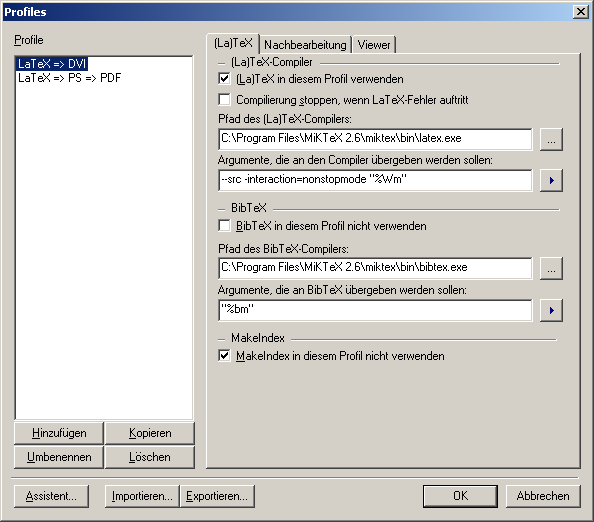
\includegraphics[width=0.49\textwidth]{techniccenter-profile-dvi-26} &
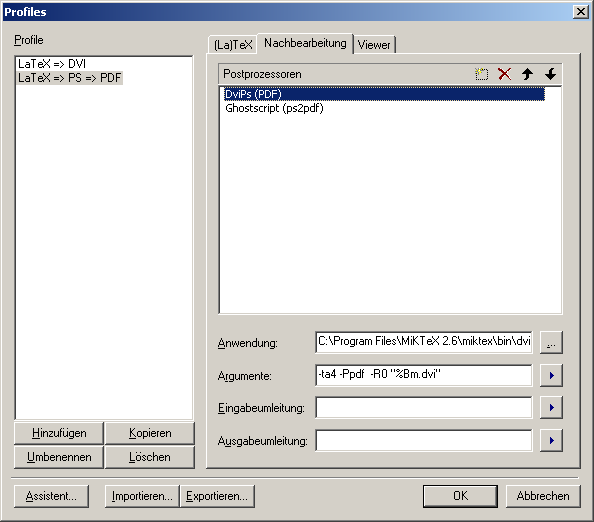
\includegraphics[width=0.49\textwidth]{techniccenter-profile-dvips-26} \\[4pt]
(a) & (b)
\end{tabular}
\caption{Spezifikation der Ausgabeprofile in TeXnicCenter.}
\label{fig:techniccenter-profile-latex}
\end{figure}

In der Datei \verb!tc_output_profiles_sumatra.tco! sind  folgende beiden "`maßgeschneiderten"' Ausgabeprofile für TexNicCenter angelegt (Import über \textsf{Build} $\rightarrow$ \textsf{Define Output Profiles ...}):
\begin{itemize}
	\item \verb!LaTeX => PDF (Sumatra)! -- Standard, direkte Erzeugung von PDF,
	\item \verb!LaTeX => PS => PDF (Sumatra)! -- PDF "`klassisch"' via DVI und PS.
\end{itemize}

\subsubsection{Profil "`\texttt{LaTeX => PDF (Sumatra)}"'}

Das ist das mit diesem Setup normalerweise verwendete Standardprofil.

\paragraph{(La)Tex:}
\begin{itemize}
  \item Path to the (La)TeX compiler: \\
        \begin{small} \verb!C:\Program Files (x86)\MiKTeX 2.9\miktex\bin\pdflatex.exe!\end{small}
  \item Command line arguments to pass to the compiler:\\
\begin{small}
   \verb!-synctex=-1 -interaction=nonstopmode "%pm"!
\end{small}
\end{itemize}

\paragraph{Postprocessor:} 
leer, kein Postprocessor notwendig.

\paragraph{Viewer:}
\begin{itemize}
\item Path of executable: \\
\begin{small}
    \verb!C:\Program Files (x86)\SumatraPDF\SumatraPDF.exe ! \\ 
    \verb!-inverse-search "\"C:\Program Files\TeXnicCenter\TEXCNTR.EXE\" !\\
    \verb!/ddecmd \"[goto('%f','%l')]\""!
\end{small}
%
\item View project's output: \\
\begin{small}
    \checkbox\ Command line argument \\\
    Command: \verb!"%bm.pdf"!
\end{small}
%
\item Forward search:\\
\begin{small}
    \checkbox\ DDE command \\\
    Command: \verb![ForwardSearch("%bm.pdf","%Wc",%l,0)]! \\
    Server: \verb!SUMATRA! \\
    Topic: \verb!Control!
\end{small}
\item Close document before running (La)TeX:\\
\begin{small}
    \checkbox\ Do not close
\end{small}
\end{itemize}


\subsubsection{Profil "`\texttt{LaTeX => PS => PDF (Sumatra)}"'}

Profil ausschließlich für den DVI-PS-Workflow (über DVI und PostScript).

\paragraph{(La)Tex:}
\begin{itemize}
  \item Path to the (La)TeX compiler: \\
        \begin{small} \verb!C:\Program Files (x86)\MiKTeX 2.9\miktex\bin\latex.exe!\end{small}
  \item Command line arguments to pass to the compiler:\\
\begin{small}
   \verb!-synctex=-1 -interaction=nonstopmode "%pm"!
\end{small}
\end{itemize}

\paragraph{Postprocessor:}
\begin{itemize}
  \item DviPS (PDF): \\
        \begin{small} 
        Executable: \verb!C:\Program Files (x86)\MiKTeX 2.9\miktex\bin\dvips.exe! \\
        Arguments: \verb!-ta4 -P pdf -R0 "%Bm.dvi"!
        \end{small}
  \item Ghostscript (ps2pdf):\\
  		\begin{small} 
        Executable: \verb!C:\Program Files (x86)\gs\gs9.04\bin\gswin32c.exe! \\
        Arguments: \verb!-q -dPDFSETTINGS=/prepress -sPAPERSIZE=a4 -dSAFER! \\
         \verb!-dBATCH -dNOPAUSE -sDEVICE=pdfwrite -sOutputFile="%bm.pdf"! \\
         \verb!-c save pop -f "%bm.ps"!
      \end{small}
\end{itemize}

\paragraph{Viewer:}
wie in Profil A. (\texttt{LaTeX => PDF (Sumatra)}).

\section{Tipps und offene Probleme:}

\begin{itemize}
\item \texttt{psfrag} funktioniert nicht mit \texttt{pdflatex} und es gibt auch leider keine Ersatzlösung. 
Wenn man \texttt{psfrag} braucht, dann muss man weiterhin über PostScript 
(\verb!LaTeX => PS => PDF!) arbeiten (was allerdings nunmehr auch mit \texttt{hyperref} kein Problem mehr ist).
%
\item Bei Verwendung des TexWorks-Editors (wird mit MikTeX ausgeliefert) sollte man die Standard-Zeichenkodierung von \emph{Unicode} (utf8) auf \emph{Latin-1} (ISO 8859-1) umstellen.
%
\item Adobe Illustrator kann beim Speichern als PDF die Bounding Box nicht setzen. 
Eine Möglichkeit ist, die Grafik zuerst als EPS zu exportieren und dann mit Acrobat in ein PDF zu konvertieren. 
%
\end{itemize}
\end{comment}



\begin{comment}
\section{Einstellungen für YAP (DVI-Viewer) im DVI-PS-Workflow}
\label{sec:YapEinstellung}

Im Standard-DVI-Viewer YAP lässt sich durch Mausklick auf das DVI-Dokument sehr leicht die zugehörige Stelle im Quelltext finden. Im Normalfall öffnet dann TeXnicCenter das zugehörige \latex-Dokument automatisch an der richtigen Stelle.
Das zugehörige "`Inverse DVI Search"' Kommando sollte sich bereits bei der Installation richtig einstellen.

Falls dies \emph{nicht} funktioniert, kann man in YAP diese Einstellung auch manuell über das Menü \textsf{View}\thinspace$\rightarrow$\thinspace\textsf{Options...} vornehmen, wie in Abb.\ \ref{fig:yap-inverse-search} gezeigt.
In diesem Fall lautet die vollständige Anweisung in "`Command Line"' folgendermaßen:
\begin{center}\footnotesize
\verb!"C:\Program Files (x86)\TeXnicCenter\TEXCNTR.EXE" /ddecmd "[goto('%f', '%l')]"!
\end{center}


\begin{figure}
\centering\small
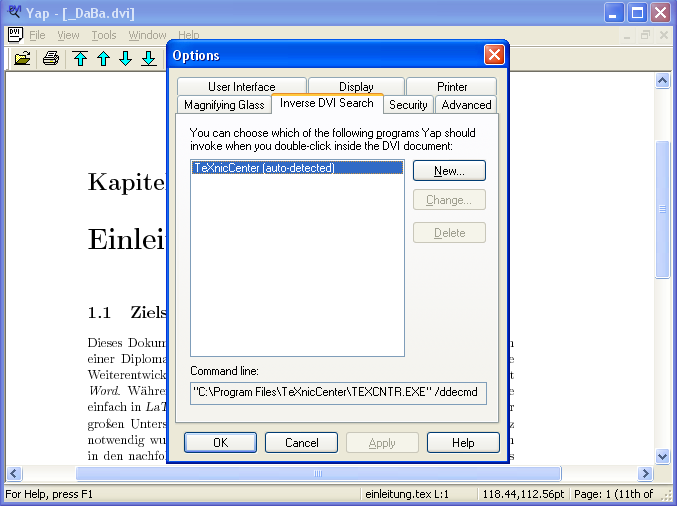
\includegraphics[width=1.0\textwidth]{yap-inverse-search-settings}
\caption{"`Inverse DVI Search"' Einstellung in YAP (über das Menü \textsf{View}\thinspace$\rightarrow$\thinspace\textsf{Options...}).}
\label{fig:yap-inverse-search}
\end{figure}

Latex
C:\Program Files\MiKTeX 2.6\miktex\bin\latex.exe
--src -interaction=nonstopmode "%Wm"

Bibtex
C:\Program Files\MiKTeX 2.6\miktex\bin\bibtex.exe
"%bm"

---

DviPs (PDF)
C:\Program Files\MiKTeX 2.6\miktex\bin\dvips.exe
-ta4 -Ppdf  -R0 "%Bm.dvi"

Ghostscript (ps2pdf)
C:\Program Files\gs\gs8.61\bin\gswin32c.exe
-sPAPERSIZE=a4 -dSAFER -dBATCH -dNOPAUSE -sDEVICE=pdfwrite -dPDFSETTINGS=/prepress -sOutputFile="%bm.pdf" -c save pop -f "%bm.ps"


YAP 
Options -> Inverse Search
"C:\Program Files\TeXnicCenter\TEXCNTR.EXE" /ddecmd "[goto('%f', '%l')]"

\end{comment}

	% Technische Ergänzungen
%\chapter{Inhalt der CD-ROM/DVD}
\label{app:cdrom}

\paragraph{Format:} 
		CD-ROM, Single Layer, ISO9660-Format%
\footnote{Verwenden Sie möglichst ein Standardformat, bei DVDs natürlich
eine entsprechende andere Spezifikation.}


\section{PDF-Dateien}
\begin{FileList}{/}
%\fitem{_DaBa.dvi} Gesamtdokument (DVI-File, ohne Grafiken)
\fitem{_thesis_DE.pdf} Master- oder Bachelorarbeit mit Instruktionen (Gesamtdokument)
\fitem{_praktikum.pdf} Praktikumsbericht (verkürzte Version der Bachelorarbeit) %
\end{FileList}


\section{\latex-Dateien}

\textbf{Achtung:} Die folgende Auflistung soll nur den Gebrauch dieser Vorlage erleichtern. Es ist bei einer Master- oder Bachelorarbeit \ia\ \emph{nicht} notwendig, die zugehörigen \latex-Dateien aufzulisten (wohl aber projektbezogene Dateien, Ergebnisse, Bilder, Kopien von Online-Literatur etc.)!

\begin{FileList}{/}
\fitem{_thesis_DE.tex} Master-/Bachelorarbeit (Hauptdokument) %
\fitem{_praktikum.tex} Praktikumsbericht (verkürzte Version der Bachelorarbeit) %
\fitem{references.bib} Literatur-Datenbank (BibTeX-File)
\end{FileList}

\begin{FileList}{/thesis_DE/front}
\fitem{vorwort.tex} Vorwort %
\fitem{kurzfassung.tex} Kurzfassung %
\fitem{abstract.tex} Abstract %
\end{FileList}

\begin{FileList}{/thesis_DE/chapters}
\fitem{einleitung.tex} Kapitel 1 %
\fitem{diplomschrift.tex} Kapitel 2 %
\fitem{latex.tex} Kapitel 3
\fitem{abbildungen.tex} Kapitel 4 %
\fitem{formeln.tex} Kapitel 5 %
\fitem{literatur.tex} Kapitel 6 %
\fitem{drucken.tex} Kapitel 7 %
\fitem{word.tex} Kapitel 8 %
\fitem{schluss.tex} Kapitel 9 %
\end{FileList}

\begin{FileList}{/thesis_DE/back}
\fitem{anhang_a.tex} Anhang A (Source Code) %
\fitem{anhang_b.tex} Anhang B (Inhalt CD-ROM) %
\fitem{anhang_c.tex} Anhang C (Liste der Änderungen) %
\fitem{anhang_d.tex} Anhang D (LaTeX-Quellcode) %
\fitem{messbox.tex} Messbox zur Druckkontrolle %
\end{FileList}

\section{Style/Class-Dateien}

\begin{FileList}{/}
\fitem{hgbthesis.cls} LaTeX Class-Datei für Master- und Bachelorarbeiten
\fitem{hgb.sty} LaTeX Style-Datei für alle Hagenberg-Dokumente
\fitem{hgbabbrev.sty} LaTeX Style-Datei mit Abkürzungs-Makros
\fitem{hgbbib.sty} LaTeX Style-Datei mit Bibiographie-Einstellungen
\fitem{hgbheadings.sty} LaTeX Style-Datei für Überschriften
\fitem{hgblistings.sty} LaTeX Style-Datei für Code-Umgebungen
\end{FileList}


\section{Sonstiges}

\begin{FileList}{/images}
\fitem{*.ai} Original Adobe Illustrator-Dateien %
\fitem{*.fh11} Original Macromedia Freehand-Dateien %
\fitem{*.jpg, *.png} Original Rasterbilder %
\end{FileList}
	% Inhalt der CD-ROM/DVD
%\chapter{Chronologische Liste der Änderungen}


Diese Auflistung wird nicht mehr aktualisiert.
Siehe \emph{Commits} auf \url{https://github.com/Digital-Media/HagenbergThesis}.



\begin{comment}
\begin{sloppypar}
\begin{description}
%
\item[2002/01/07]
\verb!\newfloat{program}! repariert (auch ohne Chapter). Dank an Werner Bailer!
%
\item[2002/03/06]
Copyright-Notice an internat.\ Standard angepasst. Dank an Karin Kosina!
%
\item[2002/07/28]
"`Studiengang"' $\rightarrow$ "`Diplomstudiengang"'
%
\item[2003/08/24]
Neues Macro: \verb!\Messbox{breite}{hoehe}! -- zur Kontrolle der 
Druckgröße ohne PS-Datei. Erweiterungen für Bakkalaureatsarbeiten
%
\item[2005/04/09]
Diverse Korrekturen: Captions von Tabellen nach oben gesetzt. 
\texttt{caption} auf neue Versionen adaptiert.
\texttt{subfig} wird nicht mehr verwendet
%
\item[2006/01/20]
Adaptiert zur Verwendung als Praktikumsbericht 
(2.\ Bakk.-Arbeit)
%
\item[2006/03/24]
Fehler in \verb!\erklaerung! beseitigt (Dank an David Schwingenschlögl)
%
\item[2006/04/06]
Verwendung von T1-Fontencoding zur besseren Silbentrennung bei 
Umlauten etc.
%
\item[2006/06/21]
Neu: Bachelorstudiengang / Masterstudiengang.
Literaturverweise auf Bakk-Arbeiten.
\texttt{upquote.sty} eliminiert (Problem mit TS1-Kodierung).
Verwende Komma (statt Punkt) als Trennzeichen in Dezimalzahlen.
%
\item[2006/09/14]
Anmerkungen zum Thema Plagiarismus.
%
\item[2007/07/16]
Ergänzungen für Code-Listings (listings) und Algorithmen 
(\texttt{algorithmicx}).
BiBTeX-Datei aufgeräumt, Verwendung der Literaturformate 
verbessert.
Komma (statt Punkt) als Trennzeichen in Dezimalzahlen wieder 
entfernt.
Verwendung der \texttt{ae}-Fonts eliminiert (\texttt{cm-super} Fonts müssen 
installiert sein, ab MikTeX 2.5). 
Beispiel für Ersetzung in EPS-Dateien mit \texttt{psfrag}.
%
\item[2007/10/04]
Version 5.90: Das Laden der Pakete \verb!inputenc! (Option \texttt{latin}) und 
\verb!graphicx! (Option \texttt{dvips})
aus der Hauptdatei in die \texttt{sty}-Datei übertragen; \texttt{upquote} funktioniert nun.
Paket \texttt{eurosym} ergänzt für Euro-Symbol (Anregung von Andreas 
Doubrava).
Problem mit \texttt{color}-package repariert (gerasterter PDF-Ausdruck).
Hinweise bzgl.\ Literatur ergänzt (\texttt{month}, \texttt{edition}),
BibTeX-Datei gesäubert.
Hinweis zum Einfügen von vertikalem Abstand zwischen Absätzen.
Mathematik aufgeräumt, Verwendung von \texttt{amsmath}, 
Fallunterscheidungen.
Diverse Änderungen bei Tabellen und Programmkode.
Beispiele für BibTeX-Angaben von Spezialquellen: Audio-CDs, 
Videos, Filme. Einbinden von Dateien mit \verb!\include{..}!
Neue Datei: \verb!_SimpleReport.tex! für kurze Reports (Projekte etc.).
%
\item[2007/11/11]
Version 5.91: Hinweise zur Einstellung der Output-Profile in
TexNicCenter, Inverse Search Einstellung in YAP im Anhang.
%
\item[2008/04/01]
Version 6.00beta -- kompletter Umbau!
Auslagerung der Doku\-menten-relevanten Teile in eine eigene 
\emph{class}-Datei (\texttt{hgbthesis.cls}) mit Optionen.
Die neue Style-Datei \texttt{hgb.sty} ist nun unabhängig vom 
Dokumententyp und nicht mehr kompatibel mit älteren Versionen!
Die Liste der Änderungen ist jetzt in der Datei \verb!_ChangeLog.tex!
(DIESE Datei) und diese wird im Anhang eingebunden.
Heading-Style auf Sans Serif geändert (ohne grausliche "`Caps"').
%
\item[2008/05/22]
Neue Vorlage für Technical Reports (Klasse \texttt{hgbreport.cls}).
Spracheinstellung nunmehr mit \texttt{babel}-Paket, Hauptsprache
des Dokuments kann als Option der Klasse angegeben werden.
Sprachumschaltung innerhalb des Dokuments funktioniert nun
richtig. Mit der Sprachoption \texttt{german} wird automatisch die neue deutsche 
Orthographie (\texttt{ngerman}) verwendet.
\texttt{babelbib} wird zur Formatierung des Literaturverzeichnisses
verwendet (neue BibTeX-Style-Optionen!).
Header werden nunmehr mit \texttt{fancyhdr}-Paket erzeugt.
Versionsnummerierung von \texttt{.cls} und \texttt{.sty} Files wird beendet 
(ab jetzt gilt: \emph{Datum} = \emph{Version}). 
%
\item[2008/06/10]
Neues Listing-Environment \texttt{PhpCode}; bei allen Listing-Eviron\-ments ist nun 
\texttt{mathescape=false} (kein Math-Mode nach \verb!$!). 
Bug bei Sprachumschaltung auf \texttt{ngerman} beseitigt.
%
\item[2008/08/15]
Diverse Kleinigkeiten in Literaturangaben überarbeitet (Dank an Norbert Wenzel), Spracheinstellung vereinheitlicht, Umlaute in \texttt{.bib}-Datei ersetzt.
%
\item[2008/10/15] 
Zusätzliche Hinweise zur MikTeX-Installation (Windows) sowie LaTeX unter Mac OS~X und Linux.
Liste der Abkürzungen ergänzt.%
\item[2008/11/15] 
Diverse Schreibfehler korrigiert (Dank an Silvia Fuchshuber). Hinweis auf 
\texttt{sloppypar}-Umgebung.
%
\item[2008/12/09] 
BibTeX-Tools: neuer Hinweis auf JabRef ergänzt, BibEdit entfernt (ist nicht mehr auffindbar).
%
\item[2009/02/09]
\texttt{hgb.sty}: Option "`\texttt{spaces}"' zu \texttt{url}-Package ergänzt (ermöglicht gezielten Zeilenumbruch in URLs). 
Im allgemeinen Setup für \texttt{listings}: \texttt{keepspaces=true};
Obsoletes Environment \texttt{sourcecode} deaktiviert.
Escape-Mode für \texttt{LaTeXCode}-Umgebung geändert.
\verb!_DaBa.tex!: Hinweis auf die Verwendung von \verb!\urldef! für die Angabe von URLs in Captions. \texttt{diplom} (statt \texttt{master}) als Standard-Dokumententyp in \verb!_DaBa.tex! ("`Diplomarbeit"'). Neuer Abschnitt zum Umgang mit ``Quellenangaben in Captions''.
\texttt{literatur.bib}: alle URLs (bisher in \texttt{note}-Einträgen) auf \verb!url={..}! geändert.
%
\item[2009/04/14]
Hinweis zum Einfügen einfacher Anführungszeichen ergänzt.
%
\item[2009/07/18]
Literaturangaben korrigiert und ergänzt.
%
\item[2009/11/27]
Experimentelle Version: Massive Änderungen, Umstieg auf \texttt{pdflatex}.
%
\item[2010/06/15]
Erstes Release der neuen Version mit \texttt{pdflatex}.
\item[2010/06/23]
Konflikt zwischen \texttt{pdfsync}-Package und \texttt{array}-Package (wird relativ häufig benutzt) durch \verb!\RequirePackage[novbox]{pdfsync}! behoben.
Seitenunterkante durch \verb!\flushbottom! fixiert,
variablen Absatzzwischenraum reduziert.
\item[2010/07/27]
Sprache der Erklärungsseite auf "`\texttt{german}"' fixiert (auch wenn die Hauptsprache des Dokuments  Englisch ist). %Datumsproblem - Hinweis von Philipp Winter
\item[2010/12/03]
Anmerkungen und Beispiele zum Zitieren von Gesetzestexten und Videos (Zeitangabe) ergänzt.
Hinweis auf \verb!\nolinkurl{..}! zur Angabe von Dateinamen.
\item[2011/01/29]
Einbau der Creative Commons Lizenz und entsprechender Hinweis in 
Abschnitt \ref{sec:HagenbergEinstellungen}. Neue Makros
\verb!\strictlicense!,
\verb!\cclicense! und
\verb!\license{...}!.
BibTeX-Einträge für Audio-CDs und Filme korrigiert, Beispiel für Online-Video ergänzt.
\item[2011/02/01]
Neues Makro \verb!\betreuerin{..}! zur Angabe einer (weiblichen) Betreuerin. 
%
\item[2011/06/26]
Umstellung der gesamten Literaturverwaltung auf \texttt{biblatex} mit dem Ziel, 
getrennte Abschnitte für verschiedene Kategorien von Einträgen im Quellenverzeichnis
zu ermöglichen. Die Wahl fiel auf \texttt{biblatex} (es gäbe andere Optionen), weil
damit BibTeX weiterhin nur einmal aufgerufen werden muss (und nicht für
mehrere Dateien). Damit verbunden sind allerdings massive Änderungen bei der
Syntax der BibTeX-Felder und es gibt auch mehrere neue Felder.
Aktuell sind 3 Kategorien von Quellen vorgesehen, entsprechende Änderungen in 
\nolinkurl{hgbthesis.cls}. Der klassische BibTeX-Workflow wird aktuell nicht
mehr unterstützt, die Möglichkeit einer künftigen Dok-Option ist aber 
vorgesehen. Das Literatur-Kapitel ist komplett überarbeitet, die .bib-Datei
wurde ausgemistet. Neu ist die Empfehlung zur Aufnahme von Bildquellen
in das Quellenverzeichnis, womit lange URLs in Captions (dort sind keine
Fußnoten möglich) nicht mehr notwendig sind. 
"`Persönliche Kommunikation"' als Literaturquelle entfernt (den Inhalt
von Interviews sollte man direkt im Anhang wiedergeben).
Das verwendete Bildmaterial wurde
erneuert, aktuell werden nur mehr Public Domain Bilder verwendet. 
Das Kapitel "`Hinweise für Word-Benutzer"' wurde endgültig entfernt.
\verb!\flushbottom! wieder auf \verb!\raggedbottom! geändert, um übermäßige 
Abstände zwischen Absätzen zu vermeiden.
%
\item[2012/05/10]
Hinweis auf die in Österreich bislang nicht zulässige Verwendung von "`Masterarbeit"'
entfernt, \texttt{master} ist nunmehr die Default-Dokumentenoption.
Anmerkungen zu lästigen \texttt{biblatex}-Warnungen ergänzt.
Angaben für Windows-Programmpfade auf Win7 angepasst, 
MikTeX 2.9 als Minimalerfordernis.\newline
Überflüssige Makros \verb!\damonat! und \verb!\dajahr! endgültig entfernt, statt
\verb!\abgabemonat! und \verb!\abgabejahr! ist nun das neue Makro
\verb!\abgabedatum{yyyy}{mm}{dd}! vorgesehen (unter Verwendung von internen Zählern).
Zur Formatierung von Datumsangaben wir das \texttt{datetime}-Paket verwendet.
\newline
Neue Fassung der eidesstattlichen Erklärung (inkl.\ englischer Version).\newline
PDF-Suche auf \texttt{synctex} umgestellt (\texttt{pdfsync}-Paket ist veraltet und
wird nun nicht mehr verwendet).
\newline
Die älteren Dateiversionen von \texttt{algorithmicx.sty} und \texttt{alg\-pseudo\-code.sty}
(bisher explizit beigefügt) wurden weggelassen.
\newline
Hinweis auf die \emph{Latin Modern Roman} OTF-Schriften ergänzt.
%
\item[2012/07/21]
Quellenverzeichnis: sprachabhängige Einstellung der Überschriften eingerichtet.
Titel des Quellenverzeichnisses auf "`Quellenverzeichnis"' (DE) \bzw\ "`References"' (EN) 
fixiert. Makro \verb!\MakeBibliography! hat damit keinen erforderlichen Parameter mehr.
%
\item[2012/09/17]
Wegen Änderungen im \texttt{biblatex}-package (Version 1.7, 2011/11/13) die Verwendung von
BibTeX als backend eingestellt (\texttt{backend=bibtex8}).
%
\item[2012/10/13]
Option \texttt{lowtilde} beim URL-package eingestellt (erzeugt \url{~} statt \verb!~!).
%
\item[2012/12/01]
In Abschnitt \ref{sec:FormatierungVonProgrammcode} zusätzliche Code-Umgebungen ergänzt:
\texttt{JsCode},
\texttt{PhpCode},
\texttt{HtmlCode},
\texttt{CssCode},
\texttt{XmlCode}.
%
\item[2012/12/08]
Die Code-Umgebungen in Abschn.\ \ref{sec:FormatierungVonProgrammcode} ergänzt und 
zur Verwendung von optionalen Argumenten erweitert (Hinweise in Abschnitt 
\ref{sec:FormatierungVonProgrammcode} auf die Argumente
\texttt{firstnumber=last} und \texttt{numbers=none}).
Quellenverzeichnis: den Eintragstyp \texttt{@software} für Games empfohlen und im Verzeichnis
der Kategorie \emph{avmedia} zugeordnet (Tab.~\ref{tab:BibKategorien} ergänzt). 
Game-Beispiel (von Manuel Wieser) und zusätzliche Tabelle \ref{tab:QuellenUndEintragstypen}
zur besseren Übersicht eingefügt.
%
\item[2013/05/17]
Wichtigste Änderung ist die vollständige Umstellung auf \textbf{UTF-8} unter Beibehaltung des 
\texttt{pdflatex}-Workflows. 
Damit sind zahlreiche weitere Modifikationen verbunden:
\newline
Alle Dateien (auch \texttt{.cls}, \texttt{.sty} und \texttt{.bib}) wurden auf UTF-8 konvertiert.
Damit sollte es auch keine Probleme mehr mit Umlauten und Sonderzeichen unter MacOS geben.
\newline
Die verwendete Standard-Schriftfamilie ist nun "`Latin Modern"' (\texttt{lmodern}). 
Sie ersetzt die "`CM-Super"' Schriften, mit denen es immer wieder Installationsprobleme gab.
Weiters wird jetzt das \texttt{cmap}-Paket zur besseren Such- und Kopierbarkeit von PDFs verwendet.
\newline
Das \texttt{listings}-Paket wurde durch \texttt{listingsutf8} ersetzt und für Umlaute im Quellcode adaptiert.
Eventuell sind weitere Adaptierungen notwendig.
\newline
\texttt{biber} (min.\ Version 1.5!) wird nun anstatt \texttt{bibtex} (unterstützt keine UTF-8 Dateien) verwendet,
zusammen mit \texttt{biblatex} (Version 2.5).
Die Anweisung \verb!\bibliography! wird (wieder) verwendet, allerdings nun in der Präambel,
um die \texttt{.bib}-Datei im Fileverzeichnis anzuzeigen.
\newline
Das Makro \verb!\C! (für die Menge der komplexen Zahlen \Cpx) musste wegen Problemen in der T1-Kodierung
ersetzt werden und heißt nun \verb!\Cpx!. Die Makros 
\verb!\R!, \verb!\Z!, \verb!\N!, \verb!\Q! und \verb!\Cpx! können nun auch außerhalb des Mathematik-Modus verwendet werden.
\newline
Der DVI-PS-PDF Workflow wird ab dieser Version überhaupt nicht mehr unterstützt. 
Damit ist auch das \texttt{psfrag}-Paket nicht mehr verwendbar. Entspechende Hinweise 
wurden aus dem Text entfernt.
\newline
\texttt{hyperref} wurde auf UTF-8 umgestellt.
Die grässlichen Standard-Rahmen und Farben der automatischen \texttt{hyperref}-Links wurden entfernt \bzw\ durch 
dezentere Farben ersetzt. Dadurch wird auch die Screen-Version der PDFs wieder lesbar.
\newline
Im Quellenverzeichnis wurde versuchsweise die \texttt{backref}-Option aktiviert. 
Damit werden bei allen Einträgen auch die zugehörigen Zitierstellen angegeben
(erscheint durchaus sinnvoll).
\newline
Die bisherigen Korrekturen zur \texttt{biblatex}-Formatierung wurden entfernt, 
alles arbeitet nun mit Standard-Einstellungen. Die ursächlichen Probleme in \texttt{biblatex}
scheinen in der aktuellen Version behoben zu sein.
\newline
Das Output-Profil für TeXnicCenter wurde für den neuen Workflow mit \texttt{biber} adaptiert und liegt nun in
\nolinkurl{_tc_output_profile_sumatra_utf8.tco}.
\newline
Das Windows-Script \verb!_clean.bat! wurde entfernt, da TeXnicCenter nun ein eigenes "`Clean Project"'-Kommando aufweist (in "`Build"').
\newline
Allgemeine Einstellungen zu \emph{headings} und \emph{biblatex} wurden aus der Datei \texttt{hgbthesis.cls} entfernt und in 
\texttt{hgbheadings.sty} \bzw\ \texttt{hgbbib.sty} verlagert. Diese können nun unabhängig verwendet werden (s.\ Beispiel in 
\texttt{\_TermReport.tex}).
\newline
Die Klassen-Datei \texttt{hgbtermreport.cls} wurde eliminiert, das Dokument \texttt{\_TermReport.tex} basiert nunmehr
auf der generischen LaTeX-Klasse \texttt{report}  und verwendet keine eigene \texttt{.cls} Datei mehr.
%
\item[2014/11/05]
Neu: Logo auf der Frontseite bei allen Dokumententypen. Dazu gibt es ein neues Kommando
\verb!\logofile{pic}!, wobei \verb!pic! der Name eine PDF-Datei im
Verzeichnis \verb!images/! ist. Falls \emph{kein} Logo erwünscht ist, 
kann man die Zeile einfach weglassen oder durch \verb!\logofile{}! ersetzen.
\newline
\texttt{hyperref}-Einstellungen: Einfärbung der Links wieder entfernt (\texttt{colorlinks = false}), weil beim Druck
nicht abschaltbar. Stattdessen einheitliche (dezente) Rahmen für alle Linkarten.
Zahlreiche Tippfehler eliminiert (Dank an Daniel Karzel).
\newline
Wegen eines Bugs in \texttt{biblatex 1.9} wurden die expliziten Abteilungen (\verb!\-!) in \texttt{literatur.bib}
vorübergehend entfernt (mit entsprechenden Folgen im Ergebnis). Der Bug soll in \texttt{biblatex 2.0} (derzeit noch
nicht verfügbar) behoben sein.
\newline
Package \texttt{color} auf \texttt{xcolor} geändert. In \texttt{hgb.sty} neues "`Convenience-Makro"' \verb!\etc! ergänzt.
Output-Profil für TeXnicCenter/SumatraPDF (Windows) repariert, forward/inverse Search funktioniert nun
(Datei \verb!_tc_output_profile_sumatra_utf8.tco!).
%
\item[2015/04/28]
Paket \texttt{subdepth} (zur verbesserten Platzierung von Sub- und Superscripts) 
in hgb.sty ergänzt.
%
\item[2015/07/14]
Hinweis und Abhilfe für die (nicht automatische) Silbentrennung in zusammengesetzten Wörtern.
Neu in \texttt{hgbheadings.sty}: \verb!\RequirePackage[raggedright]{titlesec}! verhindert Blocksatz
in Section-Überschriften (sehr unschön bei längeren Überschriften). 
Neu (in Abschn.~\ref{sec:GraphicOverlays}): Beispiel für die Verwendung des \texttt{overpic}-Pakets
zur Annotierung von importierten Grafiken (verwendet zudem das \texttt{pict2e}-Paket).
%
\item[2015/08/03]
Logo-Datei auf \texttt{logo.pdf} umbenannt.
\item[2015/09/17]
Anweisung \verb!\RequirePackage[utf8]{inputenc}! in die Doku\-menten\-dateien (\texttt{\_xxx.tex})
verschoben (auf Anregung von Markus Kohm: "`\ldots für die Verwendung von lualatex oder xelatex 
ist die Anweisung in hgb.sty störend, da bei diesen beiden aufgrund der nativen utf8-Unterstützung 
\texttt{inputenc} keinesfalls verwendet werden darf"').
\item[2015/09/19]
\texttt{hgb.sty} aufgeräumt.
Makros \verb!\@savesymbol! und \verb!\@restoresymbol! aus \texttt{hgb.sty} entfernt
(wurden nicht mehr verwendet; ggfs.\ Paket \texttt{savesym} als Ersatz).
Makro \verb!\optbreaknh! (optional break with no hyphen) auf \verb!\obnh! umbenannt.
Teile von \texttt{hgb.sty} in neue Dateien \texttt{hgbabbrev.sty} (div.\ Abkürzungen)
und \texttt{hgblistings.sty} (Code-Listings) verschoben.
Hintergrundtönung der Code-Listings heller (auf 5\% Grau) eingestellt.
Layout: \verb!\textfraction! auf 0.1 (statt fehlhafterweise 0.01) eingestellt.
\texttt{hgbbib.sty}: \verb!\clearpage! am Beginn des Quellenverzeichnisses entfernt
(für \texttt{article}-Template).
\item[2015/09/19]
Alle \texttt{.cls} und \texttt{.sty} Dateien sind jetzt ANSI-codiert (Header eingefügt), wie
laut CTAN-Richtlinien vorgesehen. Umlautzeichen wurden durch Makros ersetzt.
Nur \texttt{hgblistings.sty} ist weiterhin UTF-8 (wegen notwendiger literaler Umlaute).
\verb!\RequirePackage[utf8]{inputenc}! steht sonst nur mehr am Beginn
der jeweiligen (\texttt{.tex}) Haupttextdatei.
\item[2015/10/29]
Verwendung von "`In:"' im Quellenverzeichnis vor \texttt{article}-Einträgen
(Eigenart von biblatex) durch passendes Makro in \texttt{hgbbib.sty} unterbunden 
(Dank an S.\ Dreiseitl).
\item[2015/11/04]
Hinweise in Abschnitt \ref{sec:Software} auf TeXstudio unter Windows, Mac OS und Linux.
Release-Ausgabe.
\item[2015/12/08]
Source Directories neu strukturiert in \texttt{frontmatter}, \texttt{chapters}, 
\texttt{appendix}.
\item[2016/06/09]
Bibliography-Aliases für die Quellentypen
\texttt{video}, \texttt{movie}, \texttt{audio} und \texttt{software}
eingefügt (in \texttt{hgbbib.sty}) -- unterbindet Warnungen wegen
fehlender biblatex-Driver.
\item[2016/06/11]
Repository portiert auf GitHub (SourceForge eingefroren).  
Overleaf als experimentelle online LaTeX-Umgebung.
Hauptdateien umbenannt (auf \texttt{\_thesis}, \texttt{\_praktikum}, etc.).
\item[2016/09/28]
"`Numerierung"' auf "`Nummerierung"' geändert.
Code-Einbindung im Anhang repariert.
\item[2016/10/06]
In \texttt{hgb.sty}: Makros \verb!\Frametext! und \verb!\FramePic! eliminiert (ersetzt durch \verb!\fbox{...}!),
dazu \verb!\fboxsep! global auf Null gesetzt.
Hinweise auf \texttt{subfig}-Paket entfernt.
\item[2016/10/07]
In \texttt{hgbbib.sty}: Zeilenumbrüche bei URLs im Quellenverzeichnis werden an beliebigen Zeichen ermöglicht.
\end{description}
\end{sloppypar}
\end{comment}



%\section*{To Do} 
%\begin{itemize}
%\item Anhang B (CD-ROM Inhalt) überarbeiten -- ist nicht aktuell!
%\item Inkscape
%\item biblatex Bib-Driver für audio, video etc. ergänzen.
%\item Mathematik umbauen, typische Fehler stärker berücksichtigen (ua. Leerzeilen vor/nach Gleichungen).
%\item Literaturempfehlungen zum Schreiben von Diplomarbeiten
%\item Hinweise für Literatursuche (Bibliotheksverbund, CiteSeer,...)
%\end{itemize}





	% Chronologische Liste der Änderungen
%\chapter{\latex-Quellkode}
\label{app:latex}

\section*{Hauptdatei \texttt{\_thesis\_DE.tex}}

\paragraph{Anmerkung:}
Das sollte nur ein \emph{Beispiel} für die Einbindung von Quellcode
in einem Anhang sein. Der \latex-Quellkode der eigenen
Abschlussarbeit ist meist \emph{nicht} interessant genug, um ihn hier
wiederzugeben!

\begin{footnotesize}
\verbatiminput{_thesis_DE.tex}
\end{footnotesize}





	% Quelltext dieses Dokuments

%%%----------------------------------------------------------
\MakeBibliography                        % Quellenverzeichnis
%%%----------------------------------------------------------


%%%----------------------------------------------------------
\end{document}
%%%----------------------------------------------------------